\documentclass[final]{fhnwreport}       %[mode] = draft or final
                                        %{class} = fhnwreport, article, 
                                        %          report, book, beamer, standalone
%\usepackage{hyperref}
%\usepackage{graphicx}
%\usepackage{longtable} % To display tables on several pages
%\usepackage{geometry}
%\usepackage{listings}
\usepackage{colortbl}
\usepackage{lipsum}
\usepackage{silence}
\usepackage{subfig}
\usepackage{minted}
\WarningFilter{hyperref}{Draft mode on}
\WarningFilter{latex}{Marginpar}

% Load the package
\usepackage[toc]{glossaries}
% Generate the glossary
\makeglossaries

%%---Main Packages-----------------------------------------------------------------------
\usepackage[english, ngerman]{babel}	%Mul­tilin­gual sup­port for LaTeX
\usepackage[T1]{fontenc}				%Stan­dard pack­age for se­lect­ing font en­cod­ings
\usepackage[utf8]{inputenc}				%Ac­cept dif­fer­ent in­put en­cod­ings
\usepackage{lmodern}                    %The newer Font-Set
\usepackage{textcomp}					%LaTeX sup­port for the Text Com­pan­ion fonts
\usepackage{graphicx} 					%En­hanced sup­port for graph­ics
\usepackage{float}						%Im­proved in­ter­face for float­ing ob­jects
\usepackage{ifdraft}                    %Let you check if the doc is in draft mode

%%---Useful Packages---------------------------------------------------------------------
\usepackage[pdftex,dvipsnames]{xcolor}  %Driver-in­de­pen­dent color ex­ten­sions for LaTeX
\usepackage{csquotes}                   %Simpler quoting with \enquote{}
\usepackage{siunitx} 					%A com­pre­hen­sive (SI) units pack­age
\usepackage{listings}					%Type­set source code list­ings us­ing LaTeX
\usepackage[bottom]{footmisc}			%A range of foot­note op­tions
\usepackage{footnote}					%Im­prove on LaTeX's foot­note han­dling
\usepackage{verbatim}					%Reim­ple­men­ta­tion of and ex­ten­sions to LaTeX ver­ba­tim
\usepackage[textsize=footnotesize]{todonotes} %Mark­ing things to do in a LaTeX doc­u­ment

%%---Tikz Packages-----------------------------------------------------------------------
\usepackage{standalone}
\usepackage{tikz}
\usepackage{circuitikz}
\usetikzlibrary{arrows}
\usetikzlibrary{calc}
\usetikzlibrary{intersections}

%%---Math Packages-----------------------------------------------------------------------
\usepackage{amsmath}					%AMS math­e­mat­i­cal fa­cil­i­ties for LaTeX
%\usepackage{amssymb}					%Type­set­ting symbols (AMS style)
%\usepackage{array}						%Ex­tend­ing the ar­ray and tab­u­lar en­vi­ron­ments
%\usepackage{amsthm}					%Type­set­ting the­o­rems (AMS style)

%%---Table Packages----------------------------------------------------------------------
\usepackage{tabularx}					%Tab­u­lars with ad­justable-width columns
%\usepackage{longtable}
\usepackage{multirow}					%Create tab­u­lar cells span­ning mul­ti­ple rows
\usepackage{multicol}					%In­ter­mix sin­gle and mul­ti­ple columns

%%---PDF / Figure Packages---------------------------------------------------------------
\usepackage{pdfpages}					%In­clude PDF doc­u­ments in LaTeX
\usepackage{pdflscape}					%Make land­scape pages dis­play as land­scape
\usepackage{subfig}					    %Fig­ures di­vided into sub­fig­ures

%%---Other Packages----------------------------------------------------------------------
%\usepackage{xargs}                     %De­fine com­mands with many op­tional ar­gu­ments

%%---Bibliography------------------------------------------------------------------------
\usepackage[style=ieee,urldate=comp,backend=biber]{biblatex}
\addbibresource{literature/bibliography.bib}

%%---Main Settings-----------------------------------------------------------------------
\graphicspath{{./graphics/}}			%Defines the graphicspath
\geometry{twoside=false}				    %twoside=false disables the "bookstyle"
\setlength{\marginparwidth}{2cm}
\overfullrule=5em						%Creates a black rule if text goes over the margins => debugging




%%---User Definitions--------------------------------------------------------------------
%%Tabel-Definitions: (requires \usepackage{tabularx})
\newcolumntype{L}[1]{>{\raggedright\arraybackslash}p{#1}}    %column-width and alignment
\newcolumntype{C}[1]{>{\centering\arraybackslash}p{#1}}
\newcolumntype{R}[1]{>{\raggedleft\arraybackslash}p{#1}}

%%---Optional Package Settings-----------------------------------------------------------
%Listings-Settings: (requires \usepackage{listings}) => Example with Matlab Code
\lstset{language=Matlab,%
    basicstyle=\footnotesize\ttfamily,
    breaklines=false,%
    morekeywords={switch, case, otherwise},
    keywordstyle=\color{Blue},%
    tabsize=2,
    %morekeywords=[2]{1}, keywordstyle=[2]{\color{black}},
    identifierstyle=\color{Black},%
    stringstyle=\color{Purple},
    commentstyle=\color{Green},%
    showstringspaces=false,%without this there will be a symbol in the places where there is a space
    numbers=left,%
    numberstyle={\tiny \color{black}},% size of the numbers
    numbersep=9pt, % this defines how far the numbers are from the text
    %emph=[1]{word1, word2,...},emphstyle=[1]\color{red}
}							                            %loads all packages, definitions and settings, except bibliography (otherwise vim-latex doesn't recognise for completion)
% Some definitions
\definecolor{highlightyellow}{RGB}{250,237,39}
\definecolor{LightCyan}{rgb}{0.88,1,1}
\urldef{\gitpluginurl}\url{https://github.com/TKone7/clightning-plugins/tree/3b47ab992413d7bf9747be1320654b3478c60d37/dumpgraph}
\urldef{\github}\url{https://github.com/TKone7/ln-bachelor-thesis}

%%---Bibliography------------------------------------------------------------------------
%% \usepackage[style=ieee,urldate=comp,backend=biber]{biblatex}
%% \addbibresource{literature/bibliography.bib}

\usepackage[natbib=true, citestyle=apa, bibstyle=apa]{biblatex}
\bibliography{literature/bibliography.bib}


\title{Effectivenes simulation of a rebalancing algorithm for the Lightning Network under partial participation}                          %Project Title
\author{Bachelor Thesis}                %Document Type => Technical Report, ...
\date{August 1, 2020}                   %Place and Date

\begin{document}
%%---TITLEPAGE---------------------------------------------------------------------------
\selectlanguage{english}                %ngerman or english
\maketitle

\vspace*{-1cm}                            %compensates the space after the date line.
\vfill
{
\renewcommand\arraystretch{2}
\begin{center}
\begin{tabular}{>{\bf}p{4cm} l}
Organization                  &    FHNW, School of Business, Basel\\
Study program                 &    Business Information Technology\\
Author                        &    Tobias Koller\\
Supervisor                    &    Prof. Dr. Kaspar Riesen\\
Project sponsor               &    Prof. Dr. Thomas Hanne\\
Expert                        &    René Pickhardt
\end{tabular}
\end{center}
}
\clearpage

%% -- ABSTRACT
\thispagestyle{empty}
\begin{abstract}
  Here follows my abstract
  \lipsum{1-2}

  \vspace{2ex}
  \textbf{Keywords: Lightning, Bitcoin, path finding}
\end{abstract}
\vfill

%%---TABLE OF CONTENTS-------------------------------------------------------------------
\pagenumbering{Roman}		
\tableofcontents
\clearpage

%%---DECLARATION OF HONOR
\addcontentsline{toc}{section}{Declaration of honor}
\vfill\noindent
\begin{center}
 \section*{DECLARATION OF HONOR}
\end{center}

I the undersigned declare that all material presented in this paper is my own work or fully and specifically acknowledged wherever adapted from other sources. I understand that if at any time it is shown that I have significantly misrepresented material presented here, any degree or credits awarded to me on the basis of that material may be revoked. I declare that all statements and information contained herein are true, correct and accurate to the best of my knowledge and belief. This  paper or part of it have not been published to date. It has thus not been made available to other interested parties or examination boards.  

\vspace*{4em}\noindent
\hfill%
\begin{tabular}[t]{c}
  \rule{10em}{0.4pt}\\Tobias Koller 
\end{tabular}%
\hfill%
\begin{tabular}[t]{c}
  \rule{10em}{0.4pt}\\ Place / Date
\end{tabular}%
\hfill\strut
\clearpage

%%---FOREWORD
\section*{Foreword}
\addcontentsline{toc}{section}{Foreword}
\todo[inline]{Some background}
\clearpage

%%---GLOSSARY
\clearpage


\pagenumbering{arabic}
\section{Introduction} 
This section gives a brief introduction and overview of the Bitcoin and Lightning technology. It covers the history of digital cash, the advent of Bitcoin and explains the need for an off-chain scaling solution. 

\subsection{Bitcoin: Peer to Peer Electronic Cash}\label{subsec:peertopeer}
Bitcoin is a peer-to-peer electronic cash system first introduced in a white paper by the individual or group behind the pseudonym Satoshi Nakamoto \citep{nakamoto_bitcoin_2008}. This paper lines out the fundamental principles of the Bitcoin block chain \todo{glossary block chain} that achieves digital transfer of value without a central third party. The next paragraph expands on the pre-bitcoin developments on electronic cash that eventually lead to the rise of Bitcoin. Additionally, we explain why there is a need for additional layer protocols.

\subsubsection{History of digital cash}
Before the digital age cash was the dominant form of payment. A bank note or a coin embodies the respective face value to the bearer of it. Economical transactions can be made by simply exchanging this physical token by which the transaction was immediately settled. However, with the advent of e-commerce this simple and transparent mechanism was no longer possible. New institutions formed to fulfill the need of online transactions. Credit card companies and payment processors filled the gap of trust needed between the sender and the receiver of a transaction over the internet. This architecture came with significant drawbacks. Suddenly, the interacting parties are dependent on third parties which are collecting additional fees. Use of such systems require identification and since the intermediary can track all transactions, this reduces the user's privacy \citep{narayanan_bitcoin_2016}.

Bitcoin is by no means the first system introduced to allow for a digital cash system. Already in in 1983 \citeauthor{chaum_blind_1983} worked on new cryptographic primitives that should make electronic banking services more private and offer improved auditability \citep{chaum_blind_1983}. Although his technology still relied on a central ``bank'' server which issues electronic bills, blinded signatures allowed to anonymously transfer them. In 1989 the company \textbf{DigiCash} was found by Chaum to commercialise the idea and a few banks did later implement it. Technological complexity, patents on the invention and the incapability of handling  user-to-user transactions prevented it from becoming a success \cite{narayanan_bitcoin_2016}. 

An important problem in the evolution of digital cash has been the so called \textbf{\gls{doublespend}}. Digital information has the property of being easily duplicated. This poses a problem to digital cash as this behaviour is generally unwanted. How can a receiver of digital cash be certain that the cash has not been spent to someone else before, thus eliminating its value? Satoshi Nakamoto introduced the concept of a global distributed ledger, a data structure that is append only and where any change must be disseminated to all participants. In order to keep the history of the ledger immutable Satoshi utilizes the idea of a time stamping server first proposed by \textcite{haber_how_1991} in 1991. It works by calculating the hash of a piece of data and publishing it to all the participants. This serves as a proof that the data existed at this given time since otherwise the hash could not have been calculated. The next piece of data to be published also contains the previous hash, effectively linking them and forming a chain. If someone would now want to change the underlying data this would change its hash and since it is included in the next element in the chain also this hash would need to be changed up until the most recent element. 
\todo[inline]{explain hash and add to glossary}

Maintaining a global state of transactions in a constantly changing network of participants which can not be trusted is challenging. A single user could spin up hundreds of nodes to overcome the conses of the network. How can a consensus be formed without a central authority? A solution to a similar problem was proposed by \textcite{back_hashcash_2002} in 2002. To prevent e-mail spamming he introduced a mechanism that requires the sender to solve a puzzle that is computational heavy. This so called ``proof of work'' is requested by the receiver of the e-mail to trust that it is no spam. Since this computation can easily be done for one e-mail it becomes a big burden to do for thousand of e-mails therefore avoiding spammers. The puzzle simply involves finding a value whose hash starts with a certain amount of zero bits. Since the result of a hash function can not be predicted only brute force can be applied to find such a value. By selecting the number of leading zero bits one can change the difficulty of the puzzle. Each additional zero leads to the difficulty to be doubled. In order to add transactions to the Bitcoin ledger a participant constructs a block consisting of transactions, computes the proof of work and publishes it to the network. Only if all transactions are valid and the work done has been verified network participants append the transactions to their local copy of the ledger and further broadcast the block.  
\todo[inline]{add pow to glossary}

Combining proof of work with the chaining of hashes introduced in the last paragraph results in a strong security model. An attacker who wants to change the history of the ledger would need to recompute the proof of work of the changed and all subsequent blocks as they are linked by their hashes. Therefore, every new block makes it increasingly more difficult to change a transaction in the ledger. Number of blocks on top of a transaction in question is hence be referred to as \textbf{confirmations}.  

\subsubsection{Scaling solutions}
One of Bitcoin's value propositions is being decentralised. At the same time every transaction ever made must be distributed and stored among all network peers. It becomes obvious that some trade-off has to be made to maintain those two properties: scalability. This is often referred to as the scalability trilemma \todo{trillema in glossary} which states that in distributed systems the three objectives \textbf{security}, \textbf{decentralisation} and \textbf{scalability} can not be achieved in full extent at the same time. While two can often be achieved, there are certain trade-offs to be made in the third domain. This section is explaining why this is true for Bitcoin and what main categories of solution exist.

While decentralisation can be described on many levels we focus here on the decentralisation of validating nodes. Those are network participants that verify the blocks published by miners. Decentralisation would be best achieved if  every user of Bitcoin would run its own fully validating node \todo{add full node to glossary}to receive information about the ledger independently. On the other hand the network would be centralised when only few nodes would validate and users would need to trust those to tell the truth about the ledger state. To keep decentralisation high it is crucial to keep the hardware and network requirements as low as possible. The Bitcoin protocol restricts the amount of data to be processed to one block of 1 megabyte per 10 minutes. A full node in the network must be able to download at least 1 MB / 10 minutes in order to keep up with the tip of the chain. Lower bandwidth would cause it to get left behind without every being able to catch up. Additionally, the full node must keep the full ledger on storage. This yields to approximately 286 GB \cite{noauthor_blocks-size_nodate} at time of writing, increasing linearly in the future. This upper limit block size results in a throughput of approximately 7 transactions per second (tps) \cite{poon_bitcoin_2016}. Clearly by several orders of magnitude smaller than what it would require to become a world wide payments network. 

Bitcoin, by design, promotes security and decentralisation while sacrificing scalability. However, to be usable by everyone the scalability issue needs to be addressed. As Bitcoin is not owned by anyone there is no one party to decide on the future design decisions. This lead to a scaling debate with two ideological camps on how to progress. Scaling on-chain or scaling off-chain.

Scaling on-chain means lifting the 1 megabyte block limit, allowing for a higher transaction throughput. While this seems the most straight forward solution it can not be achieved without trade-off. As previously discussed decentralisation can only be maintained by keeping the hardware and network requirements low. Removing this restriction to allow worldwide usage would mean that nodes soon need to process hundreds of megabytes or even gigabytes per second, effectively reducing the number of nodes that can still keep up, leading to a more centralised network. 

An off-chain scaling solution describes any system that acts outside of the Bitcoin protocol but is linked to it, in a way that leverages the number of economical transactions that can be performed per single on-chain transaction. These solutions build a second layer \todo{glossary second layer} of abstraction. While still using functionality of the base layer \todo{glossary base layer} they can reduce their dependency and make their own design decisions and trade-offs based on the scalability trilemma. The Lightning Network is only one possible off-chain solution and is described in the next section in more depth. 

\subsection{Lightning technology}
The Lightning Network is a network protocol that utilizes Bitcoin as its underlying trust system. It can, therefore, be described as a ``second layer'' protocol building upon the Bitcoin ``base layer''. Bitcoin does not scale on the base layer since it was designed with security and decentralisation in mind. Off-chain solutions like Lightning are developed to facilitate more transactions on a different layer without compromising the properties of the base layer \citep{poon_bitcoin_2016}.

\subsubsection{Payment channels}
The transaction bottleneck in Bitcoin is imposed since every network participant needs to be updated about every transaction. This is required to ensure the integrity of the system and not because the transactions are of interest to the nodes. In fact they can learn very little about the parties involved in a transaction as pseudonymous public keys are used as identifiers. \citeauthor{poon_bitcoin_2016} mention in the Lightning Network Paper that as long as only two participants care about a recurring transaction there is no need to inform the entire network about it \citep{poon_bitcoin_2016}. They therefore propose that those two participants do not sent the transaction to the network but instead hold on to it and agree on their balances bilaterally. \textquote[{\cite{poon_bitcoin_2016}}, p. 4]{Micropayment channels create a relationship between two parties to perpetually update balances, deferring what is broadcast to the block chain in a single transaction netting out the total balance between those two parties.}

Opening such a payment channel requires the two parties to create an on-chain Bitcoin transaction which spends an amount of bitcoin to a 2-of-2 multisignature contract. Only both parties collaboratively can spend it from there. At the same time they create a refund transaction that spends from the multisignature contract and distributes the current balance state. However, they could broadcast this transaction instead they can also decide to hold on to it and update it at a later stage. Holding the signed Bitcoin transaction ensures that they could at any time get their balance back on-chain. Every time they wish to transact with each other they just sign a new refund transaction which distributes the updated channel balance.

\textit{Example:} Assume Alice and Bob open a payment channel and both send 0.5 BTC to a 2-of-2 multisignature contract. This channel has a total capacity of $0.5 + 0.5 = 1$ BTC. At the same time they also create a transaction that pays them back their initial balance of 0.5 BTC each. This transaction is not sent to the block chain but kept private by the two parties. If Alice wants to send Bob 0.2 BTC they update this transaction spending the initial 1 BTC to be distributed as follows: 0.3 BTC to Alice; 0.7 BTC to Bob. This payment was only agreed upon Alice and Bob, no one else needed to be notified. Unlimited future transactions like this can take place as long as the sender still has some balance. At any point in time Alice or Bob can decide to broadcast the latest transaction, distributing the agreed balance and effectively closing the payment channel. As depicted in figure~\ref{fig:ChannelCycle} there can be many modifications to that balance.

\begin{figure}[H]
\centering
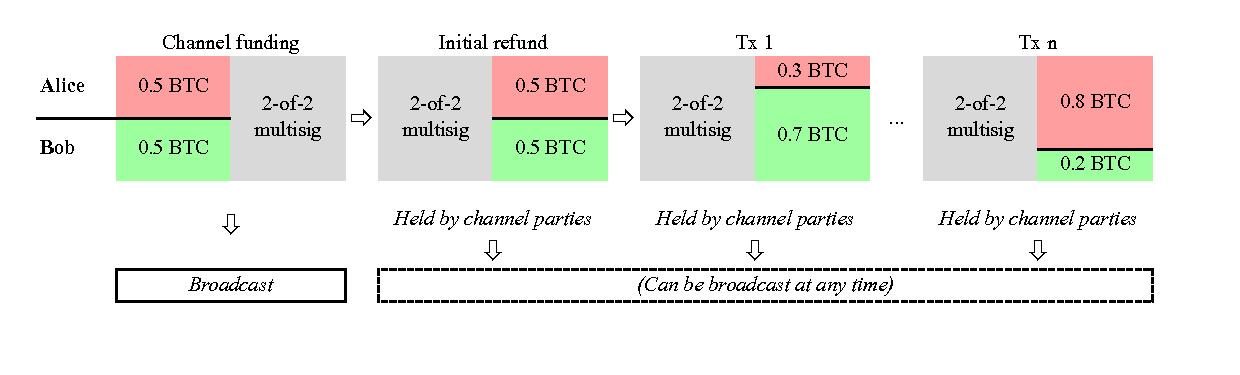
\includegraphics[width=0.9\linewidth]{channel_lifecycle.pdf}
\caption{Life cycle of payment channel.}
\label{fig:ChannelCycle}
\end{figure}

Whenever the parties decide to end there collaboration they can close the channel by broadcasting a closing transaction to the block chain which pays out each party its respective balance. While beneficial, collaborative channel closure is not required, each party can close the channel at any given time by broadcasting the latest transaction agreed upon. 

Participants in such channels are referred to as Lightning nodes, a computer system that runs an implementation of the Lightning Network protocol. Those nodes are not to be confused with Bitcoin nodes. However, since most Lightning nodes need direct access to the Bitcoin block chain most Lightning nodes are Bitcoin nodes at the same time.

\subsubsection{Using other channels for payments}
Since a payment channel is a biparty relationship an update of channel balance can only ever represent a transaction between those parties. Instead of opening a channel to each participant a node wants to transact with there is the opportunity to route payments through multiple channels.

Often economical transactions \todo{glossary econ. tx} to a specific recipient are made only once. It would therefore, defeat the purpose of Lightning to open a channel for this unique payment because both opening and closing of a channel takes each one transaction on the base block chain. Using Lightning would not use the load on-chain but rather increase it by a factor of two. This demonstrates that a payment channel should only be opened if the cost of doing so can be amortised over many transactions. This is either the case if the channel parties are expected to repeatedly transact with each other or if they can facilitate transactions between other nodes in the network through routing. 

Handling payments off-chain so far only worked between two parties that update Bitcoin transactions off-chain with the security of claiming their balance at any time on-chain. How can payments through multiple channels be accomplished without introducing trust into the system? If Alice wants to pay Carol through Bob, how can she be ensured that Bob will not keep the money and refuse to pay Carol? The solution are so called \textbf{Hash Time Locked Contracts} or short ``HTLC'' \todo{define htlc in glossary}. 

First Alice asks the payee, Carol, to create and keep a secret \textbf{R} and only share the hash of it, $hash(R)$. Alice then uses this, so called \textit{preimage} \todo{glossary preimage}, to create a special HTLC transaction that promises Bob to receive the payment amount if he has knowledge of $R$. Bob also gets informed by Alice who is next in the path to find out this secret. Bob then himself creates an HTLC with the same preimage to Carol offering her the same amount upon disclosure of $R$. Carol is the payee in the transaction and has knowledge of $R$ so she could technically claim the funds on-chain. There is however an easier solution than this. After she releases $R$, Carol and Bob can simply agree to update their channel to reflect this payment. The same is done between Alice and Bob leading to the state where all channel balances are updated and the HTLCs is rendered useless. This mechanism is called ``time locked'' because the offer of payment to the knowing $R$ is only valid for a certain timespan. If $R$ does not get released until the defined expiry the HTLC turns invalid. Therefore, it is important that each successive HTLC has a lower timespan.

\subsubsection{Routing}\label{subsec:routing}
The previous chapter explained how a payment can utilize multiple channels to reach its destination without the introduction of trust between participants. This section describes how routing takes place and what trade-off needs to be made.

To ensure privacy of payments the routing protocol uses onion routing \todo{define onion routing in glossary}. The sender of the payment encrypts the information in multiple layers so that each hop only learns about the next hop in the path. Each intermediary node only knows where the payment comes from and where it goes next. Who is the payer and the payee remains secret. Only the last node in the path finds out that it is the actual receiver of a payment.

\begin{figure}[H]
\centering
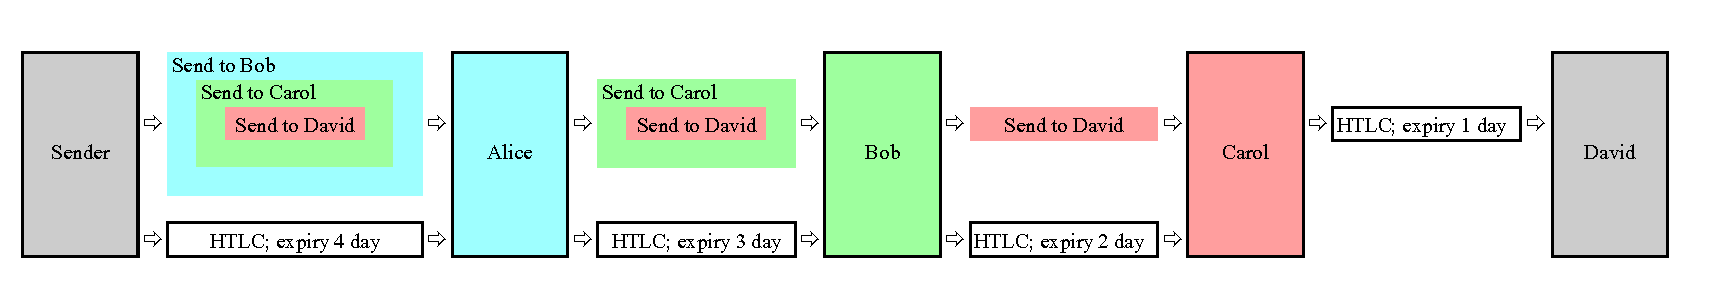
\includegraphics[width=1.0\linewidth]{htlc.pdf}
\caption{Onion routing preserves privacy over the chose path.}
\label{fig:onion}
\end{figure}

Figure~\ref{fig:onion} color codes the information which is only readable by the respective node with the same color. In each step the outermost layer is decrypted and the next hop gets revealed. The remaining encrypted data is passed on down the line. This ensures that each node only has a local view of the path knowing only about its predecessor and successor. Thus follows, the source of the payment needs to determine the complete path before sending a payment.

Sending a payment requires the sender to find a viable path to the recipient. This is called source routing \todo{glossary source routing} and necessitates some information about the channel graph. When a new channel opens the parties notify the network about the channel, its capacity and the fee policies. Each other network participants stores this information and builds up its local view of the network. When a node constructs a payment it can query a path with enough capacity along all its channels, though this is not enough to be certain that the payment can be routed. The payment in figure~\ref{fig:nopayment} of $0.5$ BTC can not be routed from Bob to Carol as Bob only owns $0.2$ BTC of the $1$ BTC channel between him and Carol. This information however is only known to Bob and Carol, not to Alice. Alice only sees the public information which tells her that the channel has 1 BTC capacity. Local channel balances are kept private for two reasons. Every payment over a channel makes its balances to move. Keeping all nodes updated about all channel balances would necessitate to update them about every transaction. This is exactly how Bitcoin on the base layer work and the reason it does not scale. Secondly, informing the Network about every transaction is very bad for privacy, as an observer could easily determine who pays to whom over what path.

Not knowing local balance distribution of channels makes it hard for source nodes to construct a reliable path. When a payment fails along the path a new route can be calculated and tried. This however is coupled with time delays that can cause a negative user experience.

\begin{figure}[H]
\centering
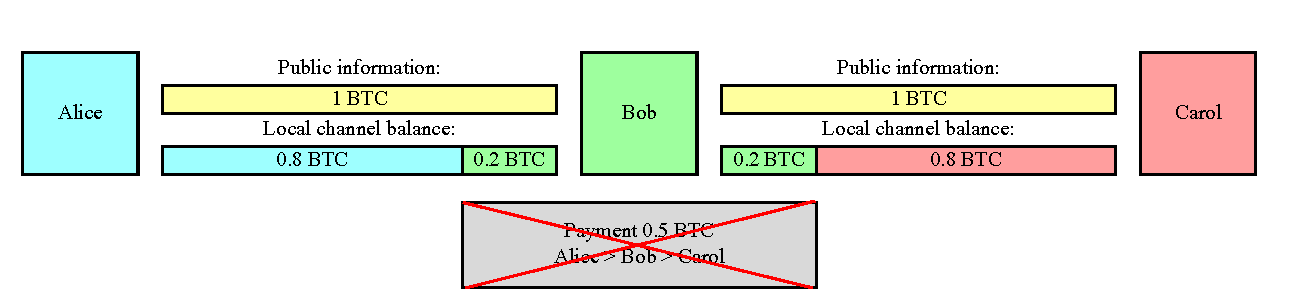
\includegraphics[width=1.0\linewidth]{nopayment.pdf}
\caption{Payment fails when channel balances cannot accommodate the required transfer.}
\label{fig:nopayment}
\end{figure}

%\newpage
\section{Problems in graph theory}
Graph theory is an old discipline which can be used to solve multifaceted problems in the real world. The following chapter contains an introduction to the basic principles and terminologies. It then defines different problems for which graph theory can be used to find solutions. More emphasis is given to the topics which are applicable to the Lightning Network.

\subsection{Formal definition}\label{subsec:formal}
The following paragraph defines the fundamentals of graph theory as described by \citet{rosen_discrete_2012}.
A graph $G=(V,E)$ consists of a set of vertices $V$ and edges $E$. An edge consists of two vertices which are called its endpoints. In an undirected graph the endpoints are unordered, whereas the pair of vertices in a directed graph are ordered. The edge $(u, v)$ of a directed graph starts at $u$ and ends in $v$. In a \textbf{simple directed} graph each directed edge can appear only once. When multiple edges go from one start vertex to the same end vertex the graph is named \textbf{directed multigraph}. An edge that connects a vertex to itself is called a loop. Assigning weights to edges allows for more complex representations mere connection and is useful if the real world representation of a connection has certain \textbf{cost} or \textbf{distance} that one might want to minimise (maximise). 

\todo[inline]{Go from general graph theory problems into more specific areas, 1 paragraph per topic}
\todo[inline]{Explain why finding a path in the lightning network can be so difficult}
\subsection{Overview of broad problems}
\todo[inline]{write an introduction to this section}

In \textbf{graph coloring problems} vertices can be thought of areas on a map. Areas that share a border are connected with an edge. The goal is to use as little colors as possible to color each area / vertex in such a way that adjacent areas have different colors. This minimum number is called the \textit{chromatic number} $\chi(G)$. 

Certain properties of graphs can only be proven if they are fulfilled in all their \textbf{subgraphs}. Hence, it is important to find those. A graph $H = (W, F)$ is a subgraph of $G = (V, E)$ when $W \subseteq V$ and $F \subseteq E$. A subgraph can be \textbf{induced} by $W \subseteq V$ which means the edge set $F$ contains only edges of $E$ for which both endpoints are contained in $W$. Similarly the union can be built of two graphs $G_1$ and $G_2$ where $G = G_1 \cup G_2$ and $V = V_1 \cup V_2$. 

Another area of graph theory aims to determine whether two graphs are \textbf{isomorphic}. This means \textquote[{\cite{rosen_discrete_2012}}, p. 668]{there is a one-to-one correspondence between their vertex sets that preserves edges.} Different algorithms are being developed that can determine isomorphism of two graphs, however with exponential worst-case time complexity. These algorithms mainly find application in chemistry and bioinformatics.  

Different \textbf{route problems} exist where the solution tries to find a path with certain properties within the graph. In the ``seven bridges of Königsberg'' the four sections of land are separated by a river and seven bridges are connecting them. The problem of passing every bridge exactly once and returning to the start can be formulated in terms of a graph with sections as vertices and bridges as edges. It is the question whether a graph has an Euler circuit or not. Many real-world applications exist where each edge needs to be visited once.

When edges have a weight assigned different problems can be modelled and optimised by finding a shortest path. A famous algorithm to find such a path is ``Dijkstra’s Algorithm''. Similarly, in the Traveling Salesperson Problem each vertex needs to be visited exactly one before returning to the starting point. Algorithms finding a path with low cost often use approximation since no algorithm with polynomial worst-case complexity exists. 

Different problems deal with the \textbf{flow} in a network. Such networks have a capacity assigned to each directed edge. Often the goal is to find the maximum flow between a source and a sink node such that all intermediary nodes have equal in and outflow \citep{even_network_1975}.

\subsection{Application in the Lightning Network}
The Lightning network can best be described by a \textbf{simple directed graph}. That is a graph with directed edges without loops and multiple directed edges. Since a payment channel between $u$ and $v$ allows payments to flow in both direction it can be modelled by use of two edges $(u, v)$ and $(v, u)$. In terms of network flow theory the capacity is the amount that can flow from $u$ to $v$ which in Lightning is defined as the local channel balance of $u$. Figure~\ref{fig:channel_graph} visualises a channel between Alice and Bob with 1 BTC capacity of which Alice holds 0.2 BTC and Bob holds 0.8 BTC.

\begin{figure}[H]
\centering
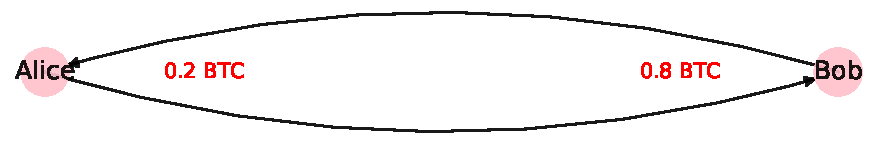
\includegraphics[width=0.9\linewidth]{simple_channel.pdf}
\caption{Lightning channel represented as simple directed graph..}
\label{fig:channel_graph}
\end{figure}

\subsubsection{Fees}
So far the properties of a network graph could be mapped to a Lightning payment channel. There is another concept within lightning that need to be accounted for. When payment channels get used by other nodes than the two channel partners they can ask for fee to be paid. This can be compared to a bridge toll that needs to be paid by everyone crossing the bridge. It is a compensation for the capital that the channel owner has ``locked''. The fee consists of two parts, a fixed fee and a variable fee. While the fixed fee is the same for every payment, the variable increases linearly with the amount being transferred.

\subsubsection{Path finding problem}
As laid out in section~\ref{subsec:routing} the initiator of a payment needs to construct the path before sending the payment. Nodes trying to find such a path work with limited information. While they know what channels are available and what their capacities are, they do not know about the balances and therefore whether the nodes can forward their payment or not. Hence, it is likely that a payment attempt fails because a node had insufficient balance. The paying node needs to find another route and retry the payment until it succeeds. If the payment fails repeatedly it can cause delays that are bad for the user experience.

This problem gets amplified because in the current protocol channels are single funded. This means one party provides 100\% of the channel capacity. A collaborative approach to funding a channel might be possible in the future. As a consequence the funder of the channel owns initially 100\% of the channel balance and the other side 0\% which means the channel can only be used to route into \textbf{one direction}. A third party trying to route through this channel has a 50:50 chance that he or she can not even route a minimal amount of 1 satoshi \todo{define satoshi and other units of btc}. 

The Lightning path finding problem can best described by a \textbf{flow network} \todo{glossary flow network}. The goal of a node constructing a payment is to find a path that has enough capacity along its channels to route to the destination. Rules from flow networks apply according to which each node, except source and sink node, must have equal amounts flowing in as are flowing out. 

In the next sections terminology native to the Lightning protocol is used. I refer to the directed graph as the \textbf{network}. Vertices are called \textbf{nodes} and a pair of opposite directed edges are a \textbf{channel}. The \textbf{capacity} defines the \textbf{total amount} of a channel which is distributed between the two node's balance, as opposed to the amount which can flow in flow networks. This flow is determined by the node's \textbf{balance}. The terms \textbf{route} or \textbf{path} are used interchangeably and are defined by a set of channels that can be traversed. \textbf{Fees} is the general term that includes both \textbf{fixed fees} and \textbf{variable fees}. Fee policies are set by each node individually for every channel. This means a channel can charge different fees in either way as both nodes set the fee policy for their balance. \textbf{Rebalancing} is the activity of routing a payment in a circle back to the initiating node and is used to reallocate balances within the set of channels a node controls.   

\subsection{Previous work}
Pickhardt's and Nowostawski's publication ``Imbalance measure and proactive channel rebalancing algorithm for the Lightning Network'' \citep{pickhardt_imbalance_2019} serves as a base to formulate the question for this thesis. In their work, they present a solution for the pathfinding problem in a privacy-aware payment channel network. The proposed solution includes a rebalancing protocol which the nodes of the network should follow to achieve a higher balancedness (for itself but also the entire network). It consists of instructions to proactively rebalance their channels within their friend of a friend's network, redistributing the relative funds owned in a channel but leaving total funds owned unchanged.

Rebalancing is an activity where one node engages in a circular payment that pays itself. This is only possible when the node has at least two channels with different peers. The payment gets routed \textbf{out} through one channel and is \textbf{received back} over another. On the way, it can use one or more hops to find back to the sender node. This procedure enables a node to change the balances of the individual channels while the total node balance stays the same. In practice, there would be a fee collected by the intermediate nodes whose channels are used. In the proposed rebalancing protocol nodes would forego the fee and only participate in the rebalancing attempt if their balancedness improves as well. The rebalancing algorithm is described in more detail in the section \todo{include ref to experiment}. 


\subsection{Problem statement}
These payment channel networks are decentralized by nature and protocol changes can not be forced upon the node operators. Therefore, the question arises on how effective this protocol change will be assuming only partial participation of nodes. What are the effects of different levels of participation on the imbalance measure \footnote{Defined as the inequality of the distribution of a nodes channel balance coefficients} of the network during repeated rebalancing cycles? What is the effect of different levels of participation on the network's ability to route payments between random nodes? 

The next part of the paper defines the rebalancing algorithm proposed in a protocol change. Then an experiment is constructed which mimics the real Lightning Network with all its participants and payment channels. I formally define multiple performance measurements which are later used to measure the improvement of the network's ability to route payments. Different scenarios are then simulated under different levels of participation also testing different ways to select the participating nodes.

\newpage
\section{Proactive Rebalancing Protocol}
\citeauthor{pickhardt_imbalance_2019} proposed in their paper a rebalancing algorithm which when proactively executed would improve the overall networks ability to route payments \citep{pickhardt_imbalance_2019}. The next sections define the algorithm in more detail and formally defines the protocol change. In later section~\ref{subsec:sim_rebal} we show how it is implemented as part of the simulation.

\subsection{Rebalancing}
Figure~\ref{fig:rebal} shows an example network with four nodes and four channels that are recently opened. The capacities are hence all on one side of the channel. Such an allocation of balances limits the use of the channels severely as they can only send payments into one direction. If Alice wants to have a better balance among her channels she can start a process called \textbf{rebalancing}. This is a self-payment which routes an amount from one of her channels through the Lightning network to another of her channels. In this example Alice decides she has excess balance in the channel with Bob and insufficient balance in the one with David.

\begin{figure}[H]
\centering
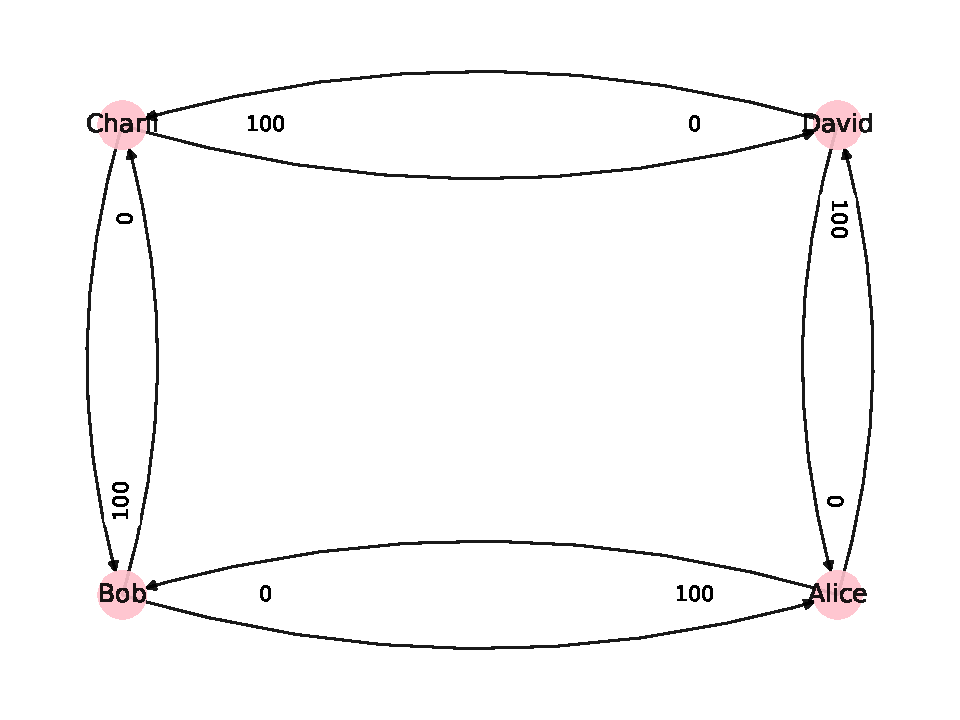
\includegraphics[width=0.9\linewidth]{rebalancing.pdf}
\caption{Initial state of newly opened channels.}
\label{fig:rebal}
\end{figure}

She can now construct a payment of e.g. 40 with the path [Alice, Bob, Charli, David, Alice]. This reduces her balance in the channel with Bob by 40 (new 60) and increases her balance in the channel with David by 40 (new 40). Both of her channels are now better balanced and allow for more payments to be routed. The resulting state is shown in figure~\ref{fig:rebal2} and the path of the rebalancing payment is indicated in red. 

This action performed by Alice did of course not only change the balances of the channels she is involved but also the ones she used to route the self-payment. In this case the channels between Bob-Charli as well as Charli-David are also more balanced. While this was the case in this example it is not guaranteed to be true in all cases, it might well be that some channels end up less balanced. The reason why all the nodes are incentivised to participate are fees that they can collect on each payment they forward. In fact they do not even know that this payment is a rebalancing transaction. Hence, Alice has to pay fees for this rebalancing operation. 

Rebalancing can be summarised as an activity performed by a single node attempting to improve the local balances of its channels by sending a payment out through one channel with excess balance and receiving it through a channel with too little balance, effectively paying itself. For all the nodes in the routing path this payment looks no different to any other payment, so they charge their normal routing fees. While the balances within the channel change a node's total balance remains constant. Alice still has a total balance of 100 allocated differently among her two channels. 

\begin{figure}[H]
\centering
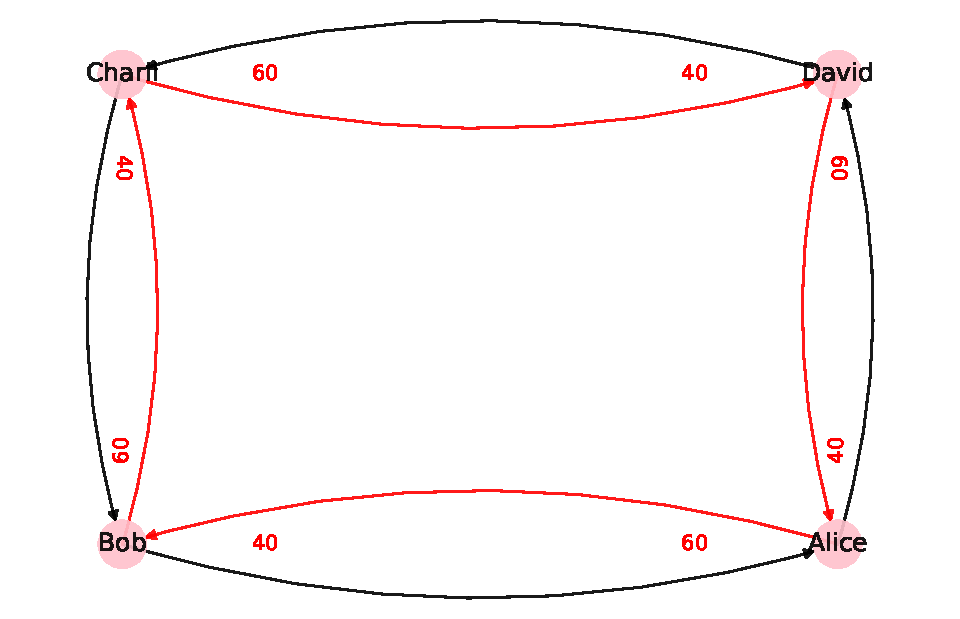
\includegraphics[width=0.9\linewidth]{rebalancing2.pdf}
\caption{Rebalancing from Alice through Bob, Charli and David.}
\label{fig:rebal2}
\end{figure}

\subsection{Rebalancing algorithm}
The previous section was about how nodes can \textit{improve} their channel balances. While the improvement in the example was quite clear it has to be stated what the ultimate goal is towards which the nodes try to improve. Intuitively, a distribution of 50:50 in each channel could be thought of as an appropriate goal. In reality this is not a feasible target.

\subsubsection{Imbalance definition}
The following terms will first be defined to better understand the problem. The two nodes in a payment channel $e=(u,v)$ are denoted as $e_u$ and $e_v$. The capacity of $e=(u,v)$ is privately split among the two nodes channel balance $b(e_u)$ and $b(e_v)$. Therefore, the capacity of the channel $c(e)=b(e_u)+b(e_v)$. The \textbf{channel balance coefficient } for $u$ represents the ratio a node $u$ has in a channel $e=(u,v)$ and is defined as $\zeta{(u,v)}=\frac{b(e_u)}{c(e)}$. Respectively, for the node $v$ the coefficient is $\zeta{(v,u)}=\frac{b(e_v)}{c(e)}$. As both balances make up the total capacity it follows  $\zeta{(u,v)} + \zeta{(v,u)}=1$. Let us define all the channels node $u$ is part of as $U=n(u)$. The \textbf{total funds} the node $u$ owns can be denoted by $\tau_u:=\displaystyle{\sum_{e\in U}b(e_u)}$. The \textbf{total capacity} of the node's channel $\kappa_u:=\displaystyle{\sum_{e\in U}c(e)}$. We can now define the \textbf{node balance coefficient} as $\nu_u = \frac{\tau_u}{\kappa_u}$.

Both $\tau_u$ and $\kappa_u$ must remain constant during rebalancing operations. This is because the rebalancing payment pays always the node itself, so the \textbf{total funds} of a node can not increase or decrease. As no new channels are opened or closed and capacities in existing channel can not be changed \textbf{total capacity} must remain constant. The initially stated goal to have a 50:50 distribution in all channels is only achievable with a \textbf{node balance coefficient} of $0.5$. As this coefficient remains constant only nodes that already have a node balance coefficient of $0.5$ could reach that state.

\citeauthor{pickhardt_imbalance_2019} had to come up with a different balance measure which is applicable to all nodes no matter what node balance coefficient they had. So they generalised the rule discussed in the previous chapter. Every channel of node $u$ should have the same \textbf{balance coefficient} $\zeta{(u,v)}$ which would then equal the \textbf{node balance coefficient} $\nu_u$. In other words, making all channel balance coefficients as similar as possible. They then defined a measure to assess how well this is achieved for a particular node. The Gini coefficient measures the inequality of a distribution. For a node $u$ with channel balance coefficients $\zeta_{(u,v_1)},\dots,\zeta_{(u,v_d)}$ they define $G_u = \frac{\displaystyle{\sum_{i\in U} \sum_{j \in U}} | \zeta_i - \zeta_j |}{2 \displaystyle{\sum_{i \in U} \sum_{j \in U} \zeta_j}}$. When all balance coefficients are equal the Gini coefficient $G_u$ turns to $0$. A value of $G_u=1$ represents the most unequal distribution \citep{pickhardt_imbalance_2019}. 

\subsubsection{Proposed algorithm}\label{subsec:prop_algo}
The proposed algorithm should be executed by each node individually. The main goal of each node is to achieve a low value of imbalance $G_u$. The node can improve its imbalance by repeatedly executing the following steps according to \cite{pickhardt_imbalance_2019}:

\begin{enumerate}
\item A node $u$ computes its node balance coefficient $\nu_u$.
\item $u$ then computes its channel balance coefficients $\zeta_{(u,v_1)},\dots,\zeta_{(u,v_d)}$.
\item All channels $e=(u,v_i)$ for which the channel balance coefficient is higher 
than its node balance coefficient, are selected as $C = \{(u,v_i) | \zeta_{(u,v_i)} - \nu_u\ > 0\}$.
\item From the candidate set $C$ a random channel $e=(u,v)$ is selected.
\item Now the node searches for a circular payment to itself along $e=(u,v)$ by choosing a path $p = [v,x_1,\dots,x_n,u]$. The amount of that payment should decrease the value of $\zeta_{(u,v)}$ to that of $\nu_u$ and can be computed as $a = c(e)\cdot (\zeta_{(u,v)}-\nu_u)$. The end of the circle should be a channel $(x_n,u)$ for which the channel balance coefficient $\zeta_{(u,x_n)}$ is smaller than the node balance coefficient $\nu_u$.
\item The node conducts the payment if all the nodes on the path $p$ agree to participate. It could happen that some nodes will only participate with a value smaller than $a$. As this is already progress $u$ will accept the suggested amount instead of being stubborn. 
\item Repeat all steps as long as the local balance coefficients are not even enough and as long as paths are found.
\end{enumerate}

\subsection{Protocol change}
Rebalancing itself is already supported in the current Lightning protocol as it includes normal payments where the sender and receiver is the same entity. However, the incentive to do so is very small. The initiating node is the one who pays the fee for the payment. A node would only do such transactions if it can expect to earn fees on the rebalanced channels that exceed the amount of fees payed for the rebalancing. 

\citeauthor{pickhardt_imbalance_2019} propose a change in the protocol to make rebalancing more explicit \citep{pickhardt_imbalance_2019}. As the proposed algorithm in the previous section~\ref{subsec:prop_algo} shows, only nodes would participate that also benefit from the rebalancing (step 6). As this would be a win-win-situation for all participating nodes they could agree to forego the fees. This change towards a \textbf{fee-free rebalancing} would incentivise nodes to do this proactively as soon as they see the opportunity to improve their balance.

Additionally, the recommend to adopt a change in the communication protocol which allows \textquote[{\cite{pickhardt_imbalance_2019}}, p. 8]{the network to work collaboratively towards achieving a good balance by locally sharing rebalancing hints}. This sharing of local channel balances would only need to be done among the local neighbourhood of a node. This is where the nodes should look for rebalancing circles and providing hints advertises willingness to rebalance in a certain direction without revealing the exact balance of the channel in question. The privacy drawbacks are minimal as balances in the local neighbourhood can easily be probed anyways \citep{tikhomirov_probing_2020}. 
 
\subsubsection{Reasons to not participate}
So far the presented algorithm sounded like a win-win-situation for everyone and there would be no discussion around adopting it. However, it is not that simple. There are different reasons why nodes would not want to participate in such a change. Some nodes might not want to forego the revenues in fee. If they decide not to participate but most other do, they still benefit from the better overall balance of the network. So, without contribution they can harvest the benefits of others who participate. 
\todo[inline]{Should I list the need of nodes to not follow the proposed Gini-approach? Because they could technically follow a different startegy and still do fee-free-balancing and hint-sharing}

\section{Experiment}\label{sec:method}
\subsection{Methodology}
This section gives an overview over the technology used and the classes created to run the experiments described in later sections. According to \citeauthor{al-taie_python_2017} Python is a general-purpose tool that becomes more and more popular in data science and graph analysis. There are many open source libraries available in the domain of analysis of complex networks, statistics and the visualisation of data \citep{al-taie_python_2017}. Furthermore the experiments in the previous paper were conducted with Python. 

\subsubsection{Python libraries}
NetworkX is a Python library that offers tools for to create, manipulate and study the structure, dynamics and function of complex networks \citep{al-taie_python_2017}. The library provides basic operations with different types of network and also implements common algorithms often used in the study of graphs.  

For all kinds of visualisation the package Matplotlib is used. It offers broad functionality to create various types of charts. Also NetworkX has some basic drawing capabilities to visualise graphs and relies on the Matplotlib package. In this thesis visualisation of graphs is not of great use and Matplotlib is mainly used for the generation of data plots \citep{al-taie_python_2017}.

Numerical computation and statistical calculations are performed using the software packages NumPy and SciPy. 

In order to reproduce the results presented in this work all Python dependencies are written down in the file \texttt{04\_Simulation/requirements.txt} on the Github repository \footnote{\github} and the \texttt{README.md} file demonstrates how to set up the execution environment.

\subsubsection{Network class}
While NetworkX provides the basic graph functionality, I need more logic to build all the Lightning specific functions. The \textbf{Network} Python class holds all these features of which I give rough overview here. All mentions of \textbf{Network} in this section refer to the Python class named like this.

Most importantly the Network is a container that holds two NetworkX graphs. The constructor of the Network class in listing~\ref{code:init} shows these two variables \mintinline{python}{G} and \mintinline{python}{flow} which will be explained in more detail later.

\begin{listing}[H]
  \begin{minted}[
    frame=single,
    framesep=3mm,
    linenos=true,
    xleftmargin=21pt,
    tabsize=4,
    breaklines=true,
    breakanywhere=true,
  ]{python}
class Network:
    def __init__(self, G, cycles4=None):
        self.G = G
        self.flow = None
	...
  \end{minted}
  \caption{Part of Network's init method.}
  \label{code:init}
\end{listing}

Figure~\ref{fig:state_network} visualises the states a Network can be in and how a Network can be exported and restored from file. The first state is a Network that went through all the preprocessing and is ready to start with an experiment of any kind. It serves as starting point for all further modifications. To ensure reproducibility of the results it is important that the same initial state is used all the time. For the very first time, this state can only be reached by parsing a channel file (\mintinline{python}{parse_clightning()}) and going through the preprocessing. The content of such a channel file and all the preprocessing steps are explained in sections~\ref{subsec:datacol} and \ref{subsec:preproc}. After this state is reached one can create a snapshot (\mintinline{python}{create_snapshot()}) which is stored to a file. In addition a fingerprint is generated and used as identifier for this specific network state. The fingerprint is calculated by hashing all the networks nodes, edges and attributes and prevents accidental load of any altered state.

Once a snapshot is generated the Network object can be recreated from there without going through the preprocessing again. The \mintinline{python}{restore_snapshot()} function takes the fingerprint as parameter and looks for the corresponding file to reload the state. 

From the initial state one experiment can be executed. Such an experiment changes the underlying network graph and stores results within the Network object. The results should then also be exported with the \mintinline{python}{store_experiment_result()} function. It allows to later restore this specific experiment by calling the \mintinline{python}{restore_results_by_name()} class method. This setup allows to run an time intensive experiment once and then create many evaluations of the result without recomputing the experiment. 

\begin{figure}[H]
\centering
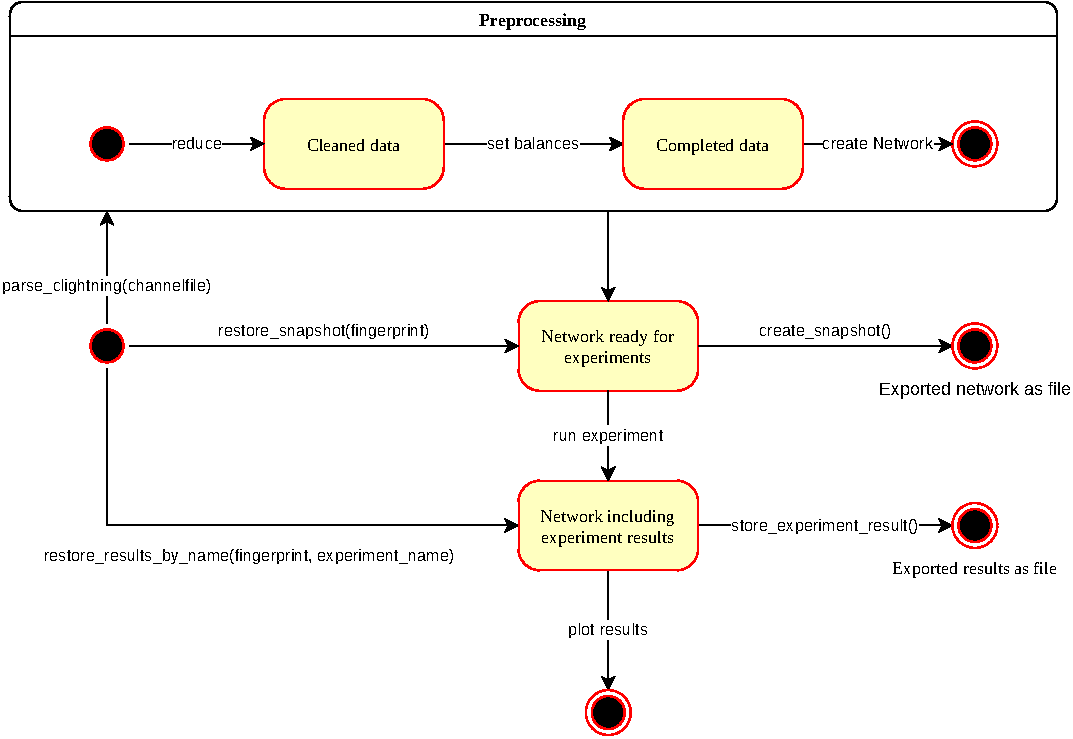
\includegraphics[width=0.9\linewidth]{state_diagram_network.pdf}
\caption{State diagram of the Network object.}
\label{fig:state_network}
\end{figure}

\subsubsection{Experiment class}
Many of the experiments actually need several Networks to perform experiments with different parameters. The experiment class is used to interact with those Network objects. This class contains also the definition of an experiment type and takes the parameters as arguments. The different \textit{setup}-methods define the types of experiments available. After the experiment is setup the generic \mintinline{python}{run_experiment()} and \mintinline{python}{plot_experiment()} can be called. Figure~\ref{fig:experiment_class} illustrates the relationship between the classes and shows the public methods of the Experiment class.

\begin{figure}[H]
\centering
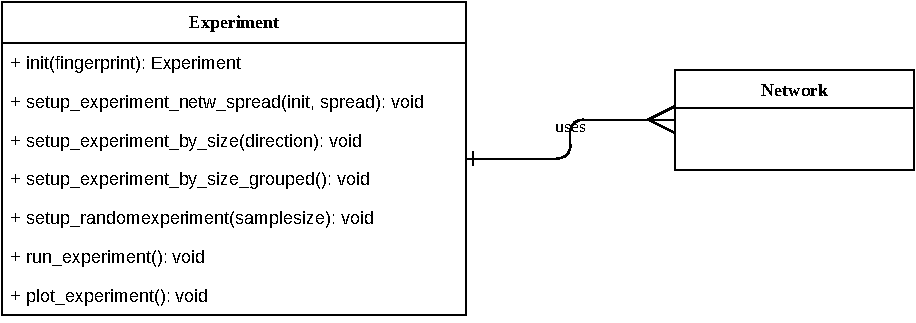
\includegraphics[width=0.7\linewidth]{experiment_network_class.pdf}
\caption{Class relationship between Experiment and Network.}
\label{fig:experiment_class}
\end{figure}

\subsubsection{Command line interface}
To simplify the interaction with the simulation software to facilitate execution of different experiment parameters without the need of changing the source code a simple command line interface can be used. The file is called \texttt{simulate.py} and uses the package \textbf{docopt} to create the interface and the parser. The interface is defines as shown in listing~\ref{code:cli}. While \texttt{parse} starts the preprocessing from a channel file all other commands execute different types of experiments and take respective parameters. The optional \texttt{---charts} flag skips the experiment and only generates the resulting charts.

\begin{listing}[H]
  \begin{minted}[
  frame=single,
  framesep=3mm,
  linenos=false,
  xleftmargin=21pt,
  tabsize=4,
  breaklines=true,
  breakanywhere=true,
]{bash}
Usage:
  simulate.py parse <filename>
  simulate.py randomexperiment <fingerprint> <samplesize> [--charts]
  simulate.py bysize <fingerprint> [(asc|desc)] [--charts]
  simulate.py groupedsize <fingerprint> [--charts]
  simulate.py spread <fingerprint> <init> <spread> [--charts]
  simulate.py -h | --help
  simulate.py --version

Options:
  -h --help     Show this screen.
  --version     Show version.
  --charts      Skips the experiment and creates only the charts.

\end{minted}
\caption{Description of the command line interface}
\label{code:cli}
\end{listing}

\subsection{Data collection}\label{subsec:datacol}
Data for the simulation was first collected from a Lightning node. This section describes the data structure obtained and what features were selected as input for the next step, the preprocessing. 

In order to run a simulation that resembles the real network closely, data from a productive Lightning node are best fitted to construct the model. Lightning is an open network which means it is easy to setup a node and download all the channel information. There are three major implementations of Lightning which technically could deliver the data. The implementation C-Lightning offers a flexible interface to write own plugins which can interact with the node over Remote Procedure Calls \todo{rpc in glossary}. I wrote a plugin \footnote{\gitpluginurl} in Python that writes all known channels to a JSON file. The code snippet~\ref{code:rawchannel} shows the raw data which is returned by C-Lightning. 

\begin{listing}[H]
\inputminted[
  frame=single,
  framesep=3mm,
  linenos=true,
  xleftmargin=21pt,
  tabsize=4,
  breaklines=true,
  breakanywhere=true,
  highlightlines={4-6,8,14-15},
  highlightcolor=highlightyellow,
]{js}{code/raw.json}
\caption{Raw channels provided by C-Lightning.}
\label{code:rawchannel}
\end{listing}

The raw data contains one key named \textbf{channels} that consists of an array. At the time of data extraction this array contained 58934 objects. Nodes can open new channels and close existing ones at any point in time. The state of the network is therefore not static. All experiments conducted in this thesis are based on the local view of my node at 30.07.2020. Each object represents one directed edge. Keys \textbf{source} and \textbf{destination} refer to the involved node's public key. This public key is used as a pseudonym to preserve the node operator's privacy. Furthermore, private public key pairs are used to encrypt (see onion routing \ref{subsec:routing}) and sign messages. Since one entry only represents one directed edge there shoud be a second entry with the same \textbf{\texttt{short\_channel\_id}} with reversed source destination nodes to make the bidirectional channel complete. Field \textbf{\texttt{sathoshis}} tells the total channel capacity in the unit ``sathoshi'' \todo{define units}. The field \textbf{\texttt{base\_fee\_millisatoshi}} is the fixed fee each payment has to pay when routing through the channel. The variable fee to pay for each million satoshis is defined by \textbf{\texttt{fee\_per\_millionth}}. All ofther fields are not important for the simulation and will be ignored. The plugin extracts the highlighted parts and writes them into a file as shown in listing~\ref{code:channelbyplugin}. 

Listing~\ref{code:channelbyplugin} shows two entries of the same \texttt{short\_channel\_id} which means they represent the same channel but in opposite directions. Source and destination of both entries confirm this and also the capacity does match. It is also an example for a channel with different fee policies in each direction. For example a payment of $200000$ satoshis routed from \textbf{02ad6f} to \textbf{03fab7} would charge no fixed fee but $\frac{200000}{1000000}*1 = 0.2$ sathoshi in variable fee. The same payment routed in the opposite direction would charge the same variable fee but additionally $1000$ millisatoshi (equals 1 satoshi) in fixed fee. So a total of $1,2$ satoshi. The complete \texttt{channels.json} file can be downloaded from the Github repository. 

\begin{listing}[H]
  \inputminted[
    frame=single,
    framesep=3mm,
    linenos=true,
    xleftmargin=21pt,
    tabsize=4,
    breaklines=true,
    breakanywhere=true
  ]{js}{code/channels.json}
  \caption{Sample channels file produced by the plugin.}
  \label{code:channelbyplugin}
\end{listing}
\subsection{Preprocessing}\label{subsec:preproc}
The date obtained in section~\ref{subsec:datacol} is not yet ready to be used to construct a network. There exist channels in the dataset for which only one of the two edges is known. Furthermore the information about the distribution of the channel balance is unknown but must be allocated somehow. These two issues are being addressed in the preprocessing which only has to be executed once. The result from the preprocessing is a \mintinline{python}{networkx.DiGraph} which is then passed to the constructor of the Network. It is then accessible through the attribute \mintinline{python}{self.G} of the Network object.

\subsubsection{Remove incomplete data}
The data sample presented in listing~\ref{code:channelbyplugin} shows that each Lightning channel is represented by two entries with opposite source-destination node pairs. In the obtained dataset not every entry has its matching counterpart. The experiments should only deal with channels that can be used in both direction (normal case), therefore, these data objects are simply deleted from the dataset. This reduced the dataset from a total of 58934 to 46366 (-6172) data objects, representing $frac{46366}{2}=23183$ channels.  

I use a \textbf{simple directed graph} to represent the Lightning network. Multiple edges with the same source and destination node are not permitted. The Lightning protocol does not prevent nodes to open multiple channels with the same partner. Therefore, multiple channels are reduced to one single channel.

\subsubsection{Allocate local balances}
The public data only contains information about the total channel capacity, the local distribution between the two channel partners is unknown. To run a simulation some distribution must be assumed. As all channels are single funded this means the capacity was all on one side initially. The best guess to distribute channel balances is therefore to assume all channels were just opened and therefore only one party hold the full capacity in its balance. However, there is no hint on who opened the channel. This is why the preprocessing allocates 100\% of the capacity to one of the parties \textbf{randomly}. To ensure reproducibility of the preprocessing the allocation of the balance should be random but deterministic. Meaning the same channel distributes the capacity to the same node in consecutive runs. Based of the evenness of the result of a hash function \todo{explain hash function} the node holding the balance is selected (see listing~\ref{code:random_alloc}).

\begin{listing}[H]
  \begin{minted}[
    frame=single,
    framesep=3mm,
    linenos=true,
    xleftmargin=21pt,
    tabsize=4,
    breaklines=true,
    breakanywhere=true,
  ]{python}
# shuffle source<->destination randomly
shuffled = set()
for channel in reduced:
    input = bytearray(channel[0] + channel[1], 'utf-8')
    hash_object = hashlib.sha256(input)
    if hash_object.digest()[0] % 2 == 0:
        shuffled.add(tuple([channel[1], channel[0]]))
    else:
        shuffled.add(channel) 
  \end{minted}
  \caption{Random allocation of channel balance.}
  \label{code:random_alloc}
\end{listing}

Depending on the allocation of the balances some nodes are not able to rebalance payments with the rest of the network. To find a network in which each node can reach each other node a NetworkX graph is created with only \textbf{one} edge pointing from the node with balance to the node without balance. From this graph the \textbf{strongly connected component} is selected. This is the directed graph in which a sequence of edges form a path from every vertex to every other vertex \citep{even_network_1975}. The resulting strongly connected component consists of 21147 channels (-2036) and has a diameter of 8. This means the longest path between any two nodes is 8.

\subsection{Simulate rebalancing}\label{subsec:sim_rebal}
In section~\ref{subsec:prop_algo} we defined the rebalancing algorithm each node following the protocol change would implement. This section demonstrates how it is implemented in the simulation. Figure~\ref{fig:flow_rebal} serves as a big picture how such a rebalancing is simulated. The next sections will go into more detail. 

\begin{figure}[H]
\centering
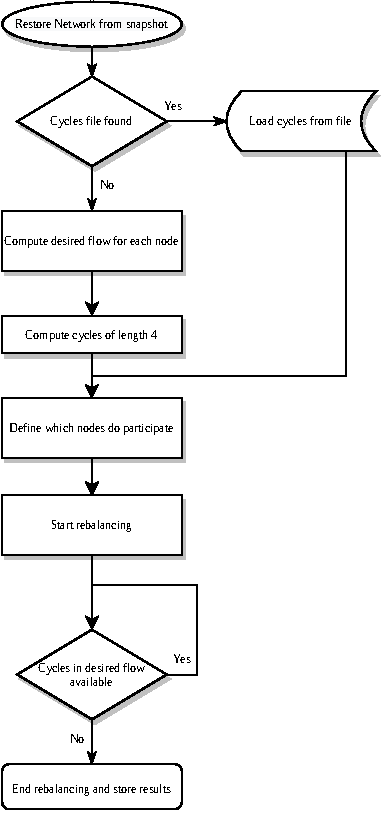
\includegraphics[width=0.7\linewidth]{flow_rebal.pdf}
\caption{Flow chart of a rebalancing experiment.}
\label{fig:flow_rebal}
\end{figure}

\subsubsection{Determine the desired flow}\label{subsub:flow}
While the rebalancing in reality would require each node to calculate the desired transactions individually we assume that rebalancing hints are shared among nodes and we can take a holistic view of the different flows each node would want to make. The method in listing~\ref{code:comp_flow} covers steps 1 to 4 and part of step 5 described in section ``\nameref{subsec:prop_algo}''.

The method \mintinline{python}{__compute_rebalance_network(self)} creates a new NetworkX graph which is derived from the original network graph (stored in \mintinline{python}{self.G}). Line 4 starts a for-loop which iterates over all edges $(u, v)$ and calculates how much node $u$ would like to send out over this edge. The first step is to calculate the node's \textbf{node balance coefficient}. This value is already pre-calculated and can be retrieved from the attributes stored in the NetworkX graph (line 7). Lines 8-10 retrieves the balance and capacity of the edge and calculates the \textbf{channel balance coefficient}. The formula from step 5 is used to calculate the amount $a = c(e)\cdot (\zeta_{(u,v)}-\nu_u)$ node $u$ would want to rebalance (line 11). This calculation returns a positive integer which represents the need to send out this amount while a negative integer represents the wish to receive this amount. 

Since a payment channel is always represented by two edges there are two nodes that have some different need to rebalance it. As the protocol foresees only rebalance transactions from which both benefit, an agreement must be found. In the case both nodes would want to rebalance into different directions (both want to send or receive at the same time) the channel is completely removed from the flow graph. As in the replicated network all channel balance lies on one end of the channel this will not be the case. However, most likely one of the nodes wants to send more than the counterparty wants to receive (or the other way around). This case is handled in lines 12-19. The lower of the two values is taken and stored into the flow graph with respect to the sign.

The result of this procedure is a property \mintinline{python}{self.flow} which contains a network graph that has two opposite directed edges for each channel that wants to be rebalanced by both parties. The amount stored in the attribute \texttt{liquidity} is the lower value the two channel partners could agree on. The value is the same for edges of a channel, but positive on the edge that wants to send and negative on the one that wants to receive. This flow graph will be used later to compute possible rebalancing paths. 

\begin{listing}[H]
  \begin{minted}[
    frame=single,
    framesep=3mm,
    linenos=true,
    xleftmargin=21pt,
    tabsize=4,
    breaklines=true,
    breakanywhere=true,
  ]{python}
 def __compute_rebalance_network(self):
        self.flow = nx.DiGraph()
        delete_edges = []
        for u, v in self.G.edges():
            if u in self.__excluded or v in self.__excluded:
                continue
            nbc = self.G.nodes[u]['nbc']
            balance = self.G[u][v]['balance']
            capacity = self.G[u][v]['capacity']
            cbc = balance / capacity
            amt = int(capacity * (cbc - nbc))
            if (v, u) in self.flow.edges():
                amt_cp = self.flow[v][u]['liquidity']
                if np.sign(amt) == np.sign(amt_cp):
                    ...
                common = min(abs(amt), abs(amt_cp))
                amt_cp = common * np.sign(amt_cp)
                amt = common * np.sign(amt)
                self.flow[v][u]['liquidity'] = amt_cp
            self.flow.add_edge(u, v, liquidity=amt)
  \end{minted}
  \caption{Method to calculate each nodes willingness to rebalance.}
  \label{code:comp_flow}
\end{listing}

\subsubsection{Compute rebalancing cycle}
Step 5 of the rebalancing algorithm tells a node $u$ to construct circular payments using a path $p = [v,x_1,\dots,x_n,u]$ for which $\zeta_{(u,v)}>\nu_u$ and $\zeta_{(x_n,u)}<\nu_u$. Such a rebalancing transaction helps a node to adjust both channel balance coefficients to the node balance coefficient. In the real network nodes would individually calculate those paths based on the \textbf{rebalancing hints} they receive from their local neighbourhood. In the simulation we already have this holistic view since we calculated the desired flow in section~\ref{subsub:flow}. 

Before we can extract the rebalancing cycles from the flow network we define the local neighbourhood of a node as the friend of a friend network. This is the network within which the proposed protocol foresees nodes to share hints about their willingness to rebalance. If we assume node \texttt{self} in figure~\ref{fig:foaf} has only two channels with \texttt{Friend1} and \texttt{Friend2}. These friends both provide information about all their channel balances (marked as green edges). This allows the node \texttt{self} to assess the rebalancing path $p = [self, Friend1, D, Friend2, self]$ with more insight about the willingness of the nodes to participate. However, this restricts the paths for rebalancing to the ones of length 4 or less. Although node \texttt{self} also knows about the channel $e = (C, X)$, it has no insight about their imbalance since it is not part of the friend of a friend network. Hence, this path of length 5 is not considered for rebalancing.

\begin{figure}[H]
\centering
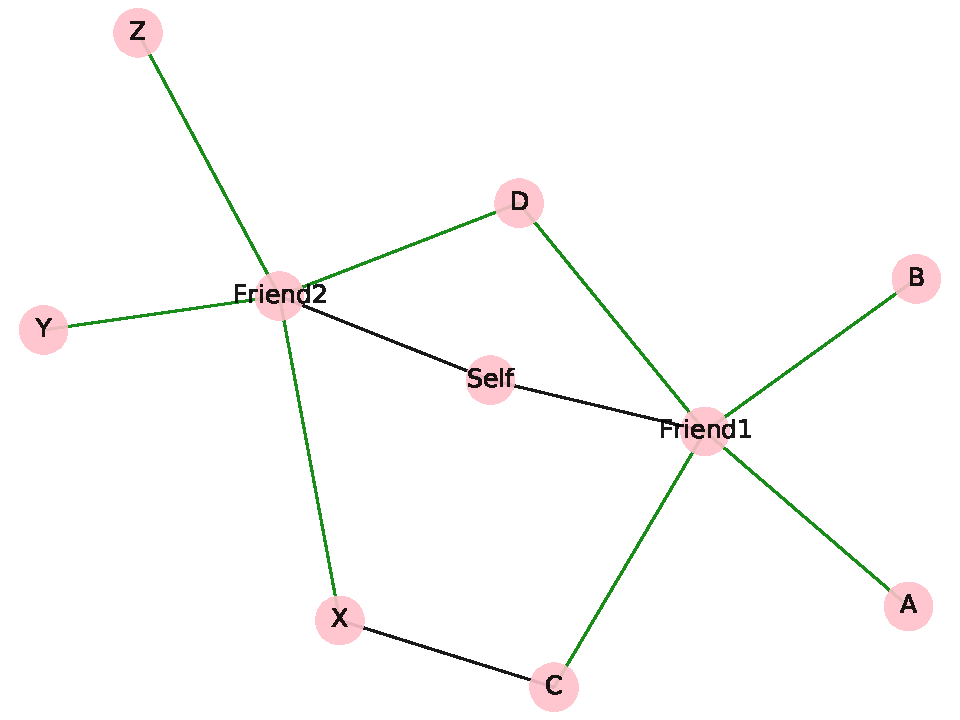
\includegraphics[width=0.9\linewidth]{foaf.pdf}
\caption{Sharing rebalance hints (green) in the friend of a friend network.}
\label{fig:foaf}
\end{figure}

The previously calculated flow network tells us the direction in which nodes want to rebalance. We can now simply extract all cycles of length 4 or less from that graph as shown in the method \mintinline{python}{compute_circles()} in listing~\ref{code:comp_circles}. 

Line 4-6 create an extract of the flow network with only positive edges. The negative edges are just the counterparts of same size in the opposite direction and can be deleted. Lines 7-9 then iterate over each edge $e = (u, v)$ and uses the built-in function \mintinline{python}{networkx.all_simple_paths()} to find all paths from $v$ to $u$. The \textbf{cutoff parameter} 3 specifies the maximum length of paths returned. To build cycles of length 4 we specify the cutoff as 3 as we add the edge $e = (u, v)$ later to make it a full circle. Since node $u$ is always the last node in the found path it does not have to be stored at this stage. All found cycles are then randomly ordered in a deterministic manner and stored to a file. 

During the future rebalancing process those set of circular paths will not change as we do not allow channels to become less balanced. This means the liquidity in the flow network only decreases and edges might disappear completely, but there is no possibility for new edges to appear. This fact is very helpful since the heavy computation of the paths needs to be done only once. If during the restore procedure an existing file of exported paths is found, this will be automatically imported.

\begin{listing}[H]
  \begin{minted}[
    frame=single,
    framesep=3mm,
    linenos=true,
    xleftmargin=21pt,
    tabsize=4,
    breaklines=true,
    breakanywhere=true,
  ]{python}
    def compute_circles(self, force=False):
        ...
        cycles4 = []
        pos_edges = [e for e in self.flow.edges(data=True) if e[2]['liquidity'] > 0]
        pos_flow = nx.DiGraph()
        pos_flow.add_edges_from(pos_edges)
        for i, (u, v) in enumerate(pos_flow.edges):
            paths = [p for p in nx.all_simple_paths(pos_flow, v, u, 3)]
            [cycles4.append(p) for p in paths if len(p) <= 4]
        ...
        self.__cycles4 = cycles4
        random.seed(10)
        self.__cycles4.sort()
        random.shuffle(self.__cycles4)
        self.__store_cycles()
  \end{minted}
  \caption{Extracts cycles of length 4 (or less) from the flow graph.}
  \label{code:comp_circles}
\end{listing}

\subsubsection{Node selection}
The main question that should be answered by the experiments is how the proposed rebalancing algorithm behaves if only a part of the entire network participates. For each level of participation an individual experiment is conducted and the nodes that should be excluded have to be defined. The selection strategies are explained in section~\ref{subsec:selstrat}.

The selection strategy is implemented in the \texttt{Experiment} class and then calls the \mintinline{python}{exclude(excl_list)} method of the Network object. The passed parameter is a list of nodes which will not participate in the rebalancing. Those nodes are stored in a local variable for later lookups. Furthermore, all the cycles which are precalculated need to be adapted. Listing~\ref{code:reduc_cyc} combines a list comprehension combined with a boolean set comparison. A set is a data structure in which each element can only be contained once. They allow for fast membership operations. Each path in \mintinline{python}{self.__cycles4} is converted to a set and then intersected with another set \mintinline{python}{self.__excluded}. If at least one of the nodes in the path is also excluded, the result is a non-empty set. Only paths with no excluded nodes in it should be kept which is checked with the boolean comparison \mintinline{python}{if not}.  

\begin{listing}[H]
  \begin{minted}[
    frame=single,
    framesep=3mm,
    linenos=true,
    xleftmargin=21pt,
    tabsize=4,
    breaklines=true,
    breakanywhere=true,
  ]{python}
def exclude(self, excl_list):
        ...
        self.__excluded = set(excl_list)
        cycles4 = [c for c in self.__cycles4 if not (set(c) & self.__excluded)]
        self.__cycles4 = cycles4
        ...
  \end{minted}
  \caption{Reduction of the available rebalancing cycles.}
  \label{code:reduc_cyc}
\end{listing}


\subsubsection{Execute rebalancing}
Once the excluded nodes are defined and the rebalancing paths are adjusted the actual rebalancing experiment can be started. In order to have results not only before and after the experiment, intermediate results are also calculated and stored. 

The \mintinline{python}{rebalance()} method start this process that runs until either no more payments can be done or the upper threshold (default: $100000$) is reached. This process iterates over all available rebalance cycles and simulates payments with the maximum possible size all nodes can agree to rebalance. This amount is found by taking the lowest \texttt{liquidity} attribute of the edges in the flow network. If this amount is at least one the rebalancing operation is executed. 

\begin{listing}[H]
  \begin{minted}[
    frame=single,
    framesep=3mm,
    linenos=true,
    xleftmargin=21pt,
    tabsize=4,
    breaklines=true,
    breakanywhere=true,
  ]{python}
def __update_channel(self, tx, rev=False):
        amount = tx[0] if not rev else tx[0] * -1
        circle = tx[1]
        for i in range(len(circle) - 1):
            src = circle[i]
            dest = circle[i + 1]
            self.G[src][dest]['balance'] -= amount
            self.G[dest][src]['balance'] += amount
            self.flow[src][dest]['liquidity'] -= amount
            self.flow[dest][src]['liquidity'] += amount
        [self.__update_node_gini(n) for n in circle[:-1]]
  \end{minted}
  \caption{Record each rebalancing payment.}
  \label{code:record}
\end{listing}

Listing~\ref{code:record} shows how a rebalancing transaction is reflected in the two networks \mintinline{python}{self.G} (state of the Lightning network) and \mintinline{python}{self.flow} (desire to rebalance). The input parameter \mintinline{python}{tx} is a tuple containing the amount and the circle. Line 4 iterates through each hop and determines the source and destination node of that hop. Since payment through a channel redistributes the local balances, both edges representing one channel have to be updated. Line 7 \& 8 increase and decrease the balances by the payment amount. Similarly the desire to rebalance represented in the flow network must be adjusted. Each payment changes the balance distribution of the involved nodes. In order to determine the new balance measure, the Gini coefficient, the \mintinline{python}{self.__update_node_gini(n)} is called for each node that was involved in the payment (line 11).

To later analyse how the network's ability to route payments improve while the network becomes more balanced, different performance measures (defined in section~\ref{sub:perfm}) are calculated. As they take a while to calculate this is not done after every payment but only when the Gini coefficient improves by $0.01$.

\subsubsection{Store and plot results}
After all rebalancing operations are performed the results should be stored to later allow to generate different data visualisations. Multiple files will be generated containing all the necessary data. The plots of the results often combine multiple networks with different participation, hence, can not be executed by the Network class. The selection of the desired data series and creation of plots is handled by the \texttt{Experiment} class.

\subsection{Performance Measures}\label{sub:perfm}
The goal of the rebalancing operations is to improve the overall networks ability to route payments between its nodes. The effectiveness of the algorithm can only be determined by measuring this ability with help of \textbf{performance measures}. This is the generic term for the measures defined in this chapter. Some of the presented indicators are also discussed in \cite{pickhardt_evaluating_2020}. 

In order to make an statement about the entire network all the presented measures consider the ability to route payments for every node in the network. As it is unclear what payments nodes would want to make, the best we can measure is one payment between each node in the network. A network with a number of nodes $N$ results in a complete payment graph with a total number of payments $N(N-1)$. The network from the experiments has 2139 nodes which results in 4575321 payments to test. This puts a limit on the computational complexity of the measures, as it becomes difficult to run the experiments on consumer hardware.

\subsubsection{Success rate on shortest path}
Successful payments between nodes is the main goal and can be measured by sending a minimal payment of 1 satoshi over all shortest paths between any two nodes. As the evaluation of the success rate is done over and over again the list of all shortest paths is cached for later use. The function \mintinline{python}{networkx.all_pairs_dijkstra_path()} is used to retrieve them. The weight to calculate short paths is represented by the fee a node would need to pay. The fee is defined by a variable and a fixed fee. As payment sizes are not known for this calculation simply the base fee is used for the shortest path calculation. 

This figure will give a good overview of how many nodes can reach each other with a minimal payment. The limitation of the measure that it does not take payment size into account and minimal payments might not be very beneficial for real payments.
%%With $E$ as the set of all shortest paths between all nodes and $P(k)$ as the proposition to route a payment of 1 satoshi over a path $k$ then the success rate is defined as:

%%$$
%%s = \frac{\displaystyle{\sum_{k \in E}} \left[ P(k) \right]}{n(E)}
%%$$

\subsubsection{Payment size on shortest path}
Similar to the success rate the \textbf{median possible payment size} also consider the shortest paths between all node pairs. On all node pairs the maximum amount that can be sent is calculated. This amount is defined by the smallest balance of all edges of the path. From all possible payment amounts the median is taken. This measure can make an assessment about how much the nodes are able to send to each other. 

\subsubsection{Ability to route different payment sizes}
Both payment size and success rate consider only the shortest path for their calculation. In reality a node that receives a payment error would simply calculate new paths and retry the payment on those. A failed payment does not necessary mean a bad user experience as several paths can be tried within a short amount of time. To account for this fact a measure should be defined that can check many paths in sequence. We define here a measure that can be seen as a combination of the latter two. 

Between each node pair not the shortest path is calculated but a set of 10 different paths. On each of those paths 3 payments of different sizes are tried to be executed. A \textbf{1-satoshi payment}, a \textbf{micro payment} of 10'000 satoshi and a \textbf{normal payment} of 100'000 satoshi. Each node pair then receives a score between 1 and 10 per payment size depending of how many paths could route the payment. The median of all node pairs then gives an indication about how successful different payment sizes are considering multiple paths in sequence. 

\subsection{Selection strategies}\label{subsec:selstrat}
The simulation will rebalance the same network with different levels of participation. This is done since it can be assumed that not all nodes will adopt a new protocol immediately. The network is not homogeneous in regards to the centrality and the degree of the nodes. The distribution of the payment channels appears to follow a power law distribution. However, we did not test distribution to actually be power-law, since \textquote[\cite{clauset_power-law_2009}, p. 1]{the detection and characterization of power laws is complicated by the large fluctuations that occur in the tail of the distribution}. But it shows a few nodes have many channels and most of the nodes only a few as can be seen in figure~\ref{fig:channelcount}. The result of the experiment, therefore, will vary depending how the participating nodes are selected. 

\begin{figure}[H]
\centering
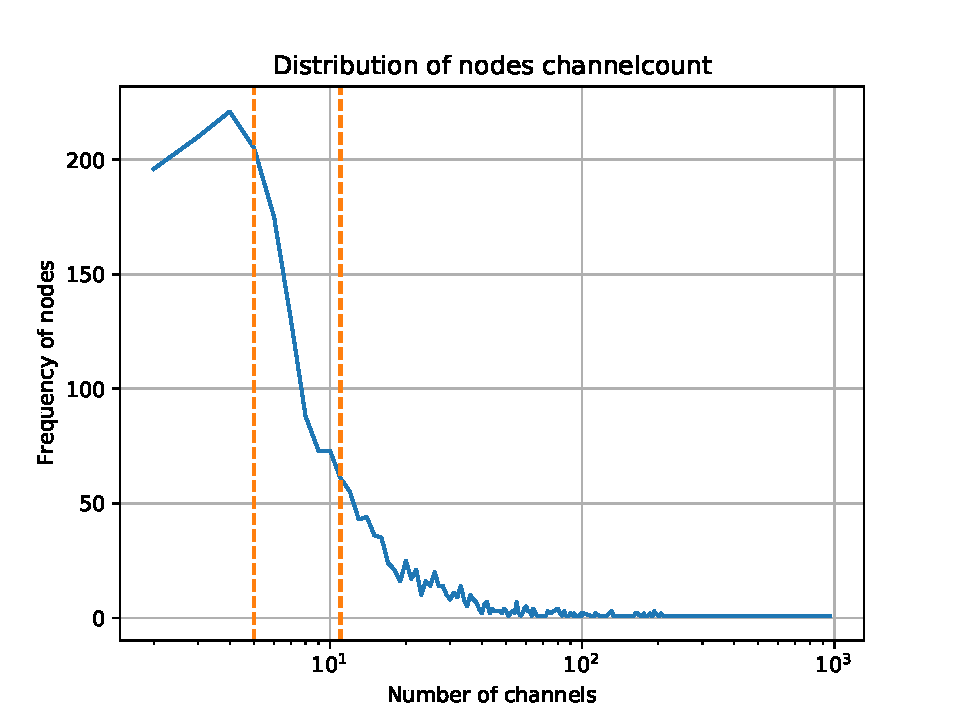
\includegraphics[width=0.7\linewidth]{channel_count_distr.pdf}
\caption{Probability distribution of the channel count of a node.}
\label{fig:channelcount}
\end{figure}

\subsubsection{Randomised}
This selection method randomly chooses $x\%$ of nodes. For value $x$, an intervals of 10 is used (10\%, 20\%, \ldots, 90\%, 100\%). The set of nodes in a smaller participation are subsets of the larger ones. To make the experiments reproducible the \mintinline{python}{random} package is seeded with a fixed value. There is a disadvantage in this method. Multiple random selections with different randomness result in other results. It could be that by coincidence a disproportionate amount of either large or small nodes are selected. In order to reduce this effect the experiment runs 10 samples with different randomness. Then from all the success measures are being averaged. 

\subsubsection{Node ranking}
The main characteristic by which we can distinguish the nodes is their importance. This can be measured in many ways. This section shows some ways how the node's importance could be determined. In a preliminary experiment we want to see if there is a significant difference.

The \textbf{degree centrality} is an easy to calculate measure. It simply counts the degree - the number of edges connected to a node. The higher the value, the more central a node is \citep{golbeck_analyzing_2013}.

A slightly more sophisticated measure is the \textbf{betweenness centrality}. It \textquote[\cite{golbeck_analyzing_2013}]{measures how important a node is to the shortest paths through the network}. A higher value means the node has an important location in the flow of information through the network. For the reason of simplicity no special weights were used for the shortest path calculation. Which means each edges was weighted equally.

The \textbf{eigenvector centrality} does not treat each neighbour equally. A node's importance will rise if it is surrounded by other important nodes. It can also be interpreted as a node's influence on the network \citep{golbeck_analyzing_2013}. A variation of eigenvector specialised for directed networks is \textbf{pagerank}. There the in-degree of influential nodes is increases the score for a node. For the Lightning network in this experiment this does not make much sense, since all nodes connected with a payment channel are connected with two edges, one in each direction.

All these different methods return a score for each node by which one could make a ranking from least to most important. We want to proof the hypothesis that for the dataset at hand all rankings would be similar. In order to compare different rankings a rank correlation can be calculated which measures the similarity of two rankings. Spearman's correlation is an appropriate way to test a monotonic relationship between two variables \citep{noauthor_resources_nodate}. It is not required for the distribution to be normal. The variables simply have to be on an ordinal scale. The resulting correlation coefficient lays between $-1$ and $1$ and is a measure for how strong the two rankings correlate. $0$ means no correlation while $1$ and $-1$ stand for strong positive or negative correlation. Table \ref{tab:spearman} shows the result of the conducted experiment. All coefficients are fairly close together, therefore, these different ranking criteria all end up with a very similar ranking. We from now on use the degree centrality as a measure for importance since it is the simplest to calculate.

\begin{table}[H]
\centering
\begin{tabular}{c | cccc} 
{} & {Degree centr.} & {Betweenness centr.} & {Eigenvector centr.} & {Pagerank} \\ \hline 
{Degree centr.} & {1.0} & {0.845} & {0.916} & {0.988} \\ 
{Betweenness centr.} & {0.845} & {1.0} & {0.698} & {0.893}\\
{Eigenvector centr.} & {0.916} & {0.698} & {1.0} & {0.880} \\
{Pagerank} & {0.988} & {0.893} & {0.880} & {1.0} \\
\end{tabular}
\caption{Ranking correlation coefficients of importance measures.}
\label{tab:spearman}
\end{table}

There are two ways to simulate different levels of participation based on this rank. Either select $x\%$ of the \textbf{top} or \textbf{bottom} as participants. 

\subsubsection{Node categories}
Similar as in the previous experiment the degree centrality is taken as a measure for a node's importance. This ranked list is then split up in three categories. The boundaries between the groups are determined by equal frequency binning to ensure equal sized groups of 713 nodes in each group. Then participation levels from 10\% to 100\% are executed for each category individually. This means 100\% participation of one group yields in a total of 33\%. 

Figure~\ref{fig:eqfreq} shows those boundaries in two different charts. Figure (a) is a cumulative histogram of the node degree (with logarithmic scale). The boundaries fall on a node degree of 5 and 11. Figure (b) shows those same boundaries but with regards to how many channels those nodes contribute. It is clearly visible that the number of channels are mainly concentrated in the last group. 

\todo[inline]{maybe declare that this was not a good boundary since one third of the smallest node have very little channels}


\begin{figure}[t]
\centering
\subfloat[Distribution of node degree]{
  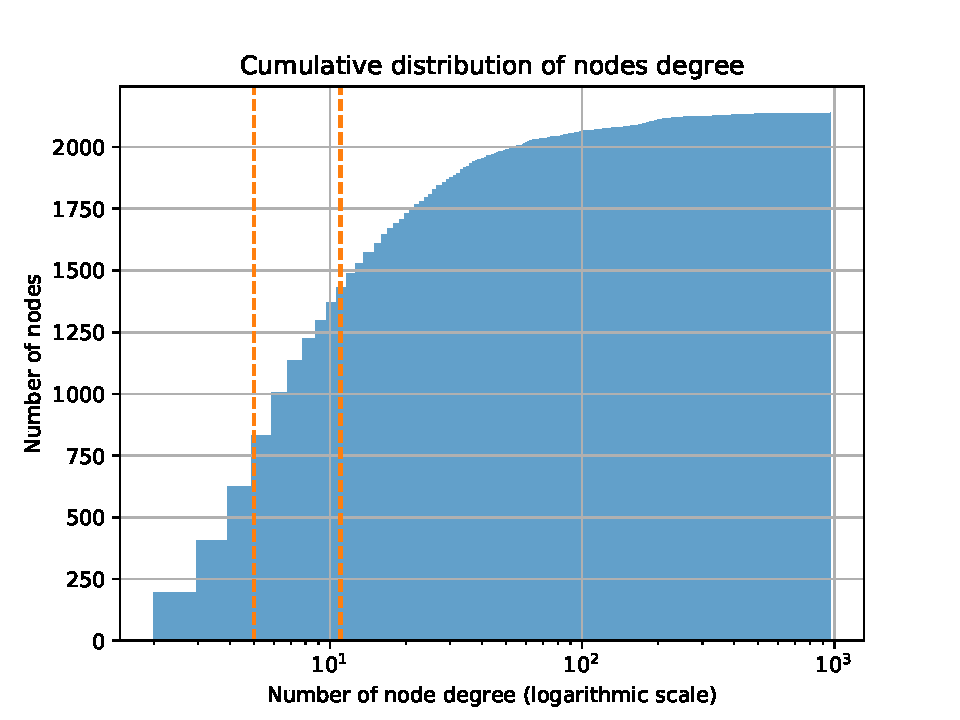
\includegraphics[width=0.45\linewidth]{cum_channel_distr_eq_width.pdf}
}\quad
\subfloat[Node's contribution to channels]{
  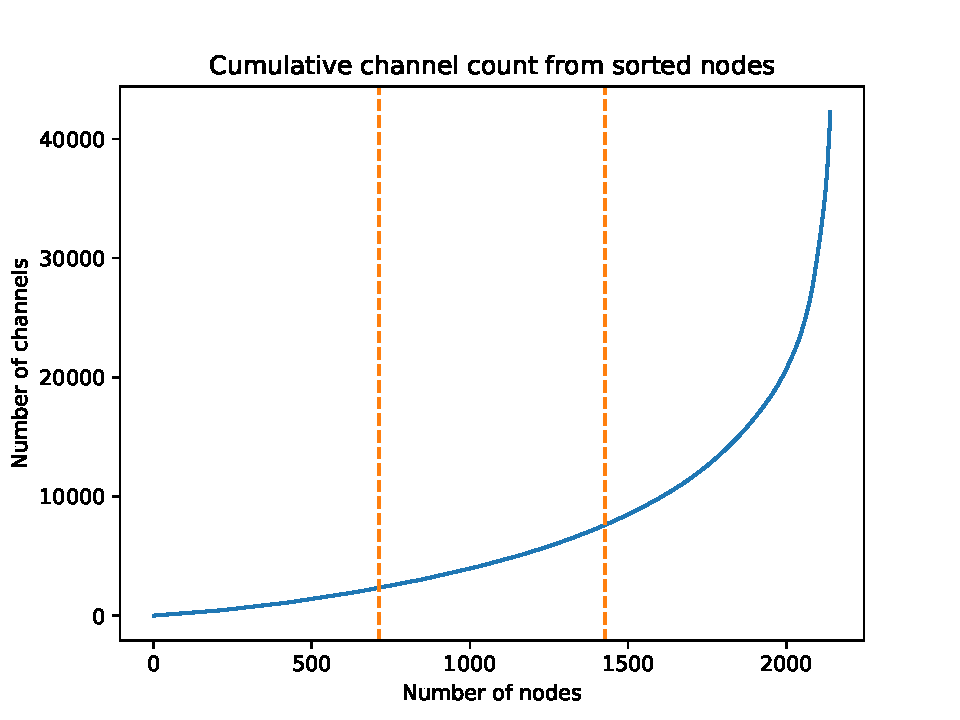
\includegraphics[width=0.45\linewidth]{node_count_to_contr_channel_count_eq_width.pdf}
}
\caption{Shows boundary definition by equal frequency.}
\label{fig:eqfreq}
\end{figure}


\subsubsection{Network spread}
For this node selection method we assume that the adoption of the new protocol is being spread through the network. Nodes only start adopting it when someone in their neighbourhood has adopted it. The simulation, therefore, starts with an initial set of nodes which participate in round 1. In each iteration a certain percentage of their channel partner participate as well. This results in two parameters which can be adjusted to simulate the way adoption can take place. \textbf{Init parameter} in \% defines how many nodes start while \textbf{spread parameter} in \% define how many of the adjacent nodes participate in the next round. Those two parameters should be chosen in a way that allows a number of participation levels similar to the 10 levels seen in the previous sections. Table~\ref{tab:param} shows the number of iterations required to reach either 99\% or 100\% of all nodes. The colored columns and row illustrate the chosen parameters which where used. An initial value of 2/10/15 \% and a spread of 40/50/60 \% result in total 9 experiments which all reach 99\% of the nodes within 7 to 11 iterations.

\newcolumntype{a}{>{\columncolor{LightCyan}}c}
\begin{table}[b]
\centering
\begin{tabular}{c|cacccccaac} 
  \multicolumn{11}{c|}{\textbf{Spread vs. Initial participation}} \\
{} & {1\%} & {2\%} & {3\%} & {4\%} & {5\%} & {7\%} & {9\%} & {10\%} & {15\%} & {20\%}  \\ \hline
{20\%} & {} & {} & {} & {24/50} & {} & {} & {23/33} & {21/33} & {22/38} & {23/50} \\
{30\%} & {} & {15/31} & {14/32} & {15/28} & {15/23} & {15/30} & {14/31} & {16/25} & {14/23} & {14/20} \\
\rowcolor{LightCyan}
{40\%} & {12/23} & {\textbf{11/20}} & {11/21} & {11/18} & {11/23} & {11/17} & {11/18} & {\textbf{11/15}} & {\textbf{11/23}} & {10/20} \\
\rowcolor{LightCyan}
{50\%} & {9/15} & {\textbf{9/13}} & {9/13} & {9/16} & {9/18} & {9/15} & {9/15} & {\textbf{9/15}} & {\textbf{8/12}} & {8/15} \\
\rowcolor{LightCyan}
{60\%} & {8/12} & {\textbf{7/12}} & {9/10} & {8/14} & {7/11} & {7/10} & {7/11} & {\textbf{7/10}} & {\textbf{7/9}} & {7/10} \\ \hline

\end{tabular}
\caption{Shows number of iterations needed to achieve 99\% or 100\% for the two parameters.}
\label{tab:param}
\end{table}

\section{Results}
Show a lot of charts :-)
\newpage
\newgeometry{left=1cm,right=0.1cm}
\begin{figure}
\begin{tabular}{ccc}
  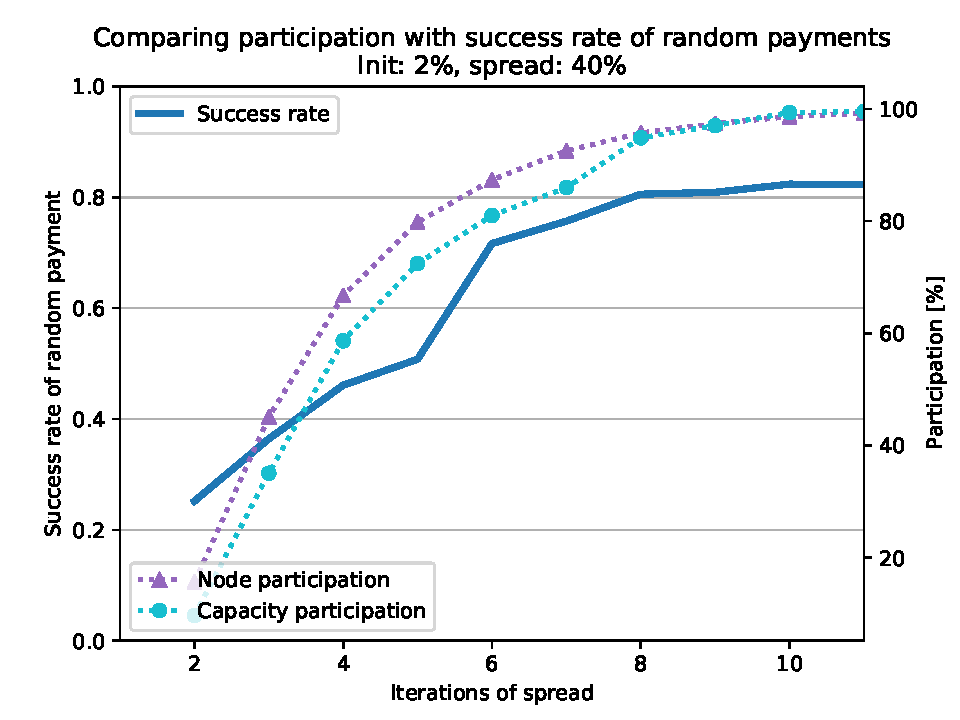
\includegraphics[width=60mm]{3a65a961_successrate_vs_participation_netw_spread_02_40.pdf} &   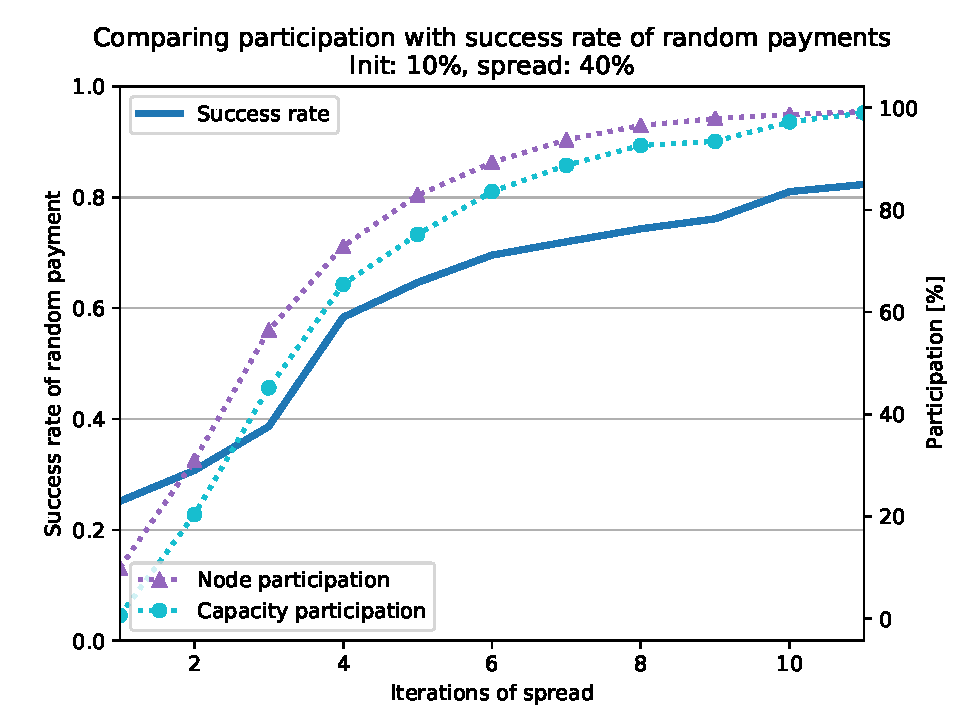
\includegraphics[width=60mm]{3a65a961_successrate_vs_participation_netw_spread_10_40.pdf} & 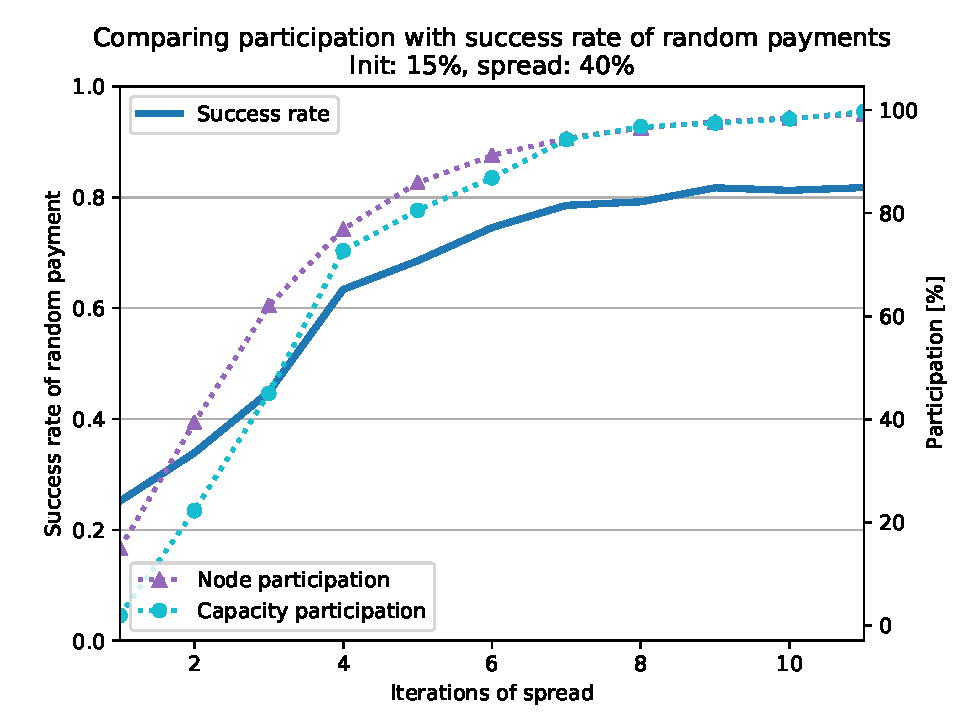
\includegraphics[width=60mm]{3a65a961_successrate_vs_participation_netw_spread_15_40.pdf}  \\
  (a) Init: 2 Spread: 40  & (b) Init: 10 Spread: 40 & (c) Init: 15 Spread: 40  \\[6pt]
  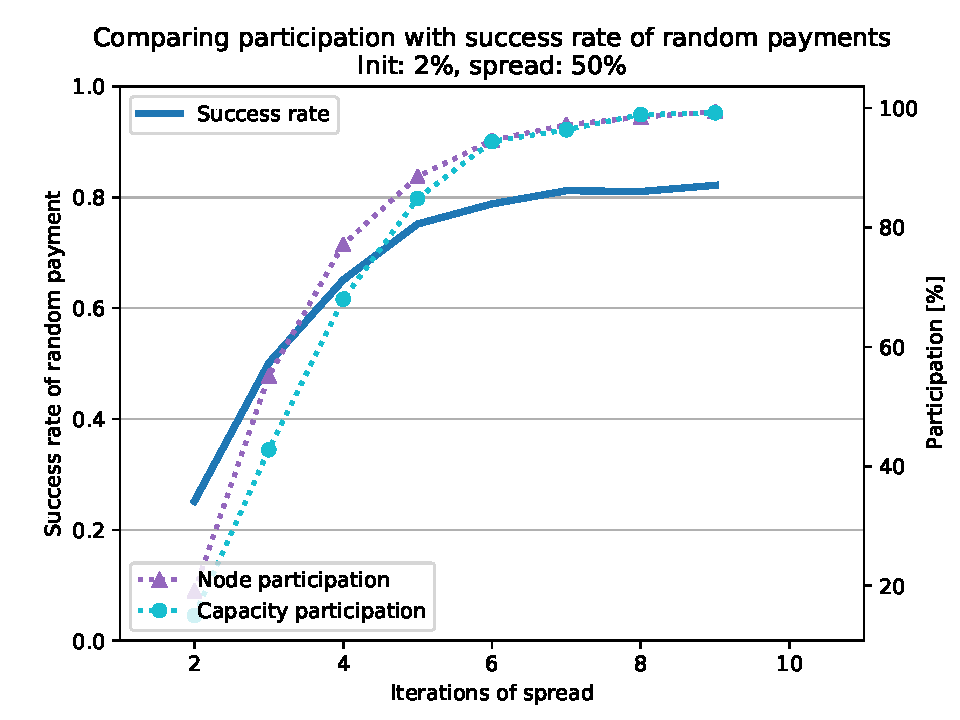
\includegraphics[width=60mm]{3a65a961_successrate_vs_participation_netw_spread_02_50.pdf} &   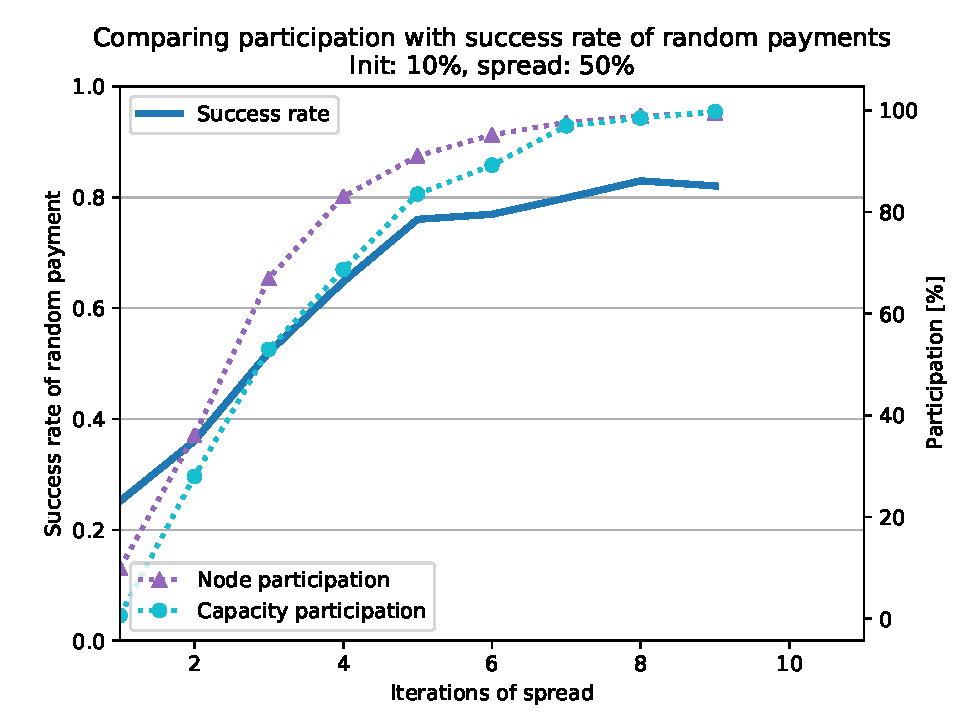
\includegraphics[width=60mm]{3a65a961_successrate_vs_participation_netw_spread_10_50.pdf} & 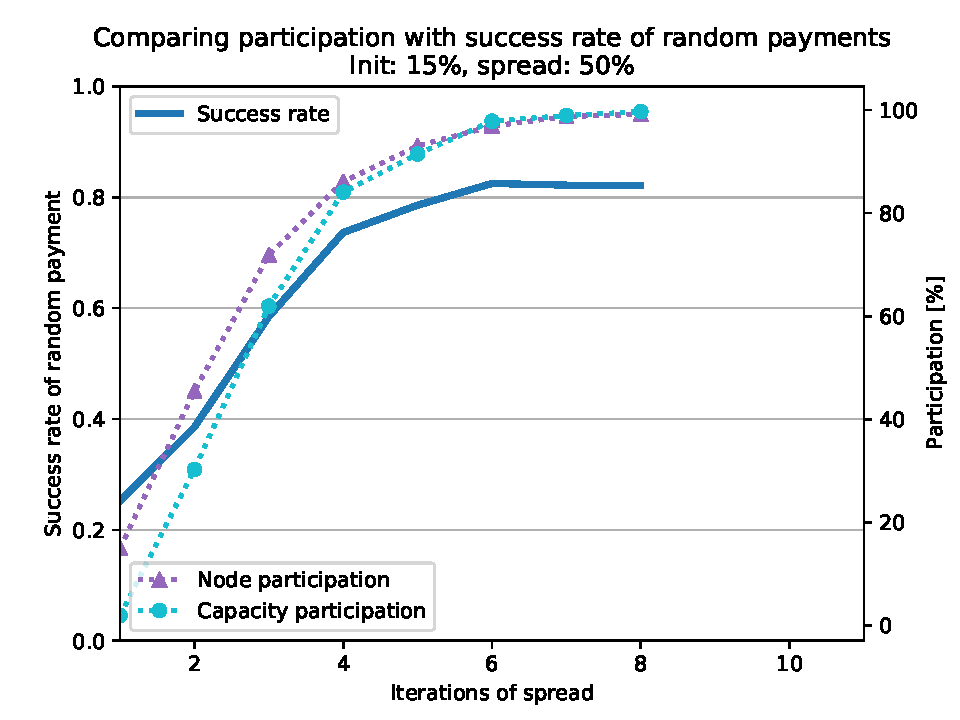
\includegraphics[width=60mm]{3a65a961_successrate_vs_participation_netw_spread_15_50.pdf}  \\
  (d) Init: 2 Spread: 50  & (e) Init: 10 Spread: 50 & (f) Init: 15 Spread: 50  \\[6pt]
  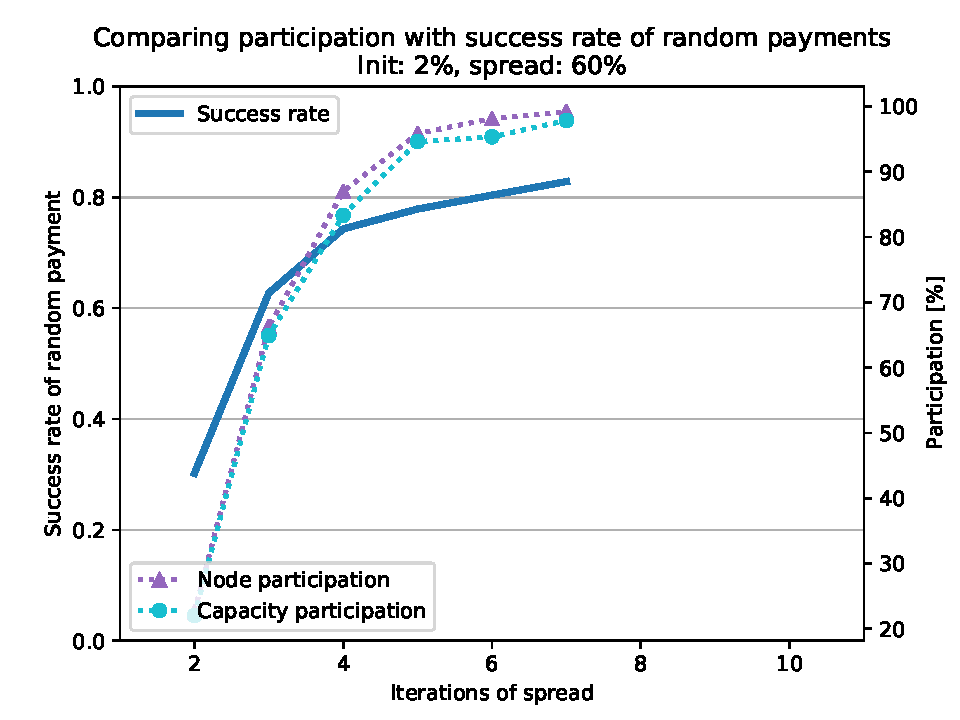
\includegraphics[width=60mm]{3a65a961_successrate_vs_participation_netw_spread_02_60.pdf} &   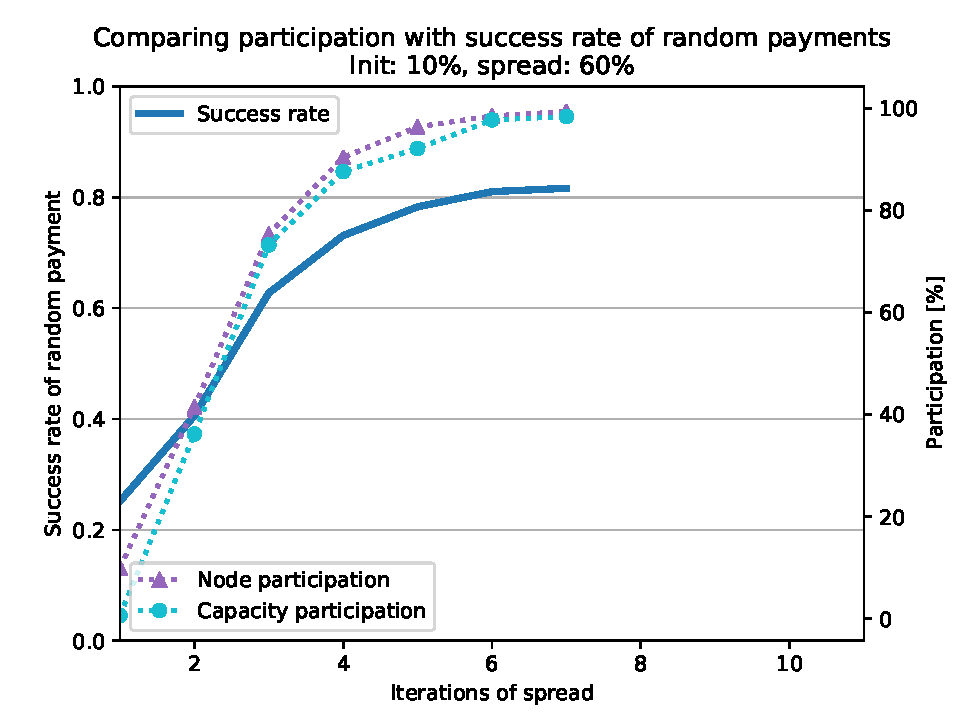
\includegraphics[width=60mm]{3a65a961_successrate_vs_participation_netw_spread_10_60.pdf} & 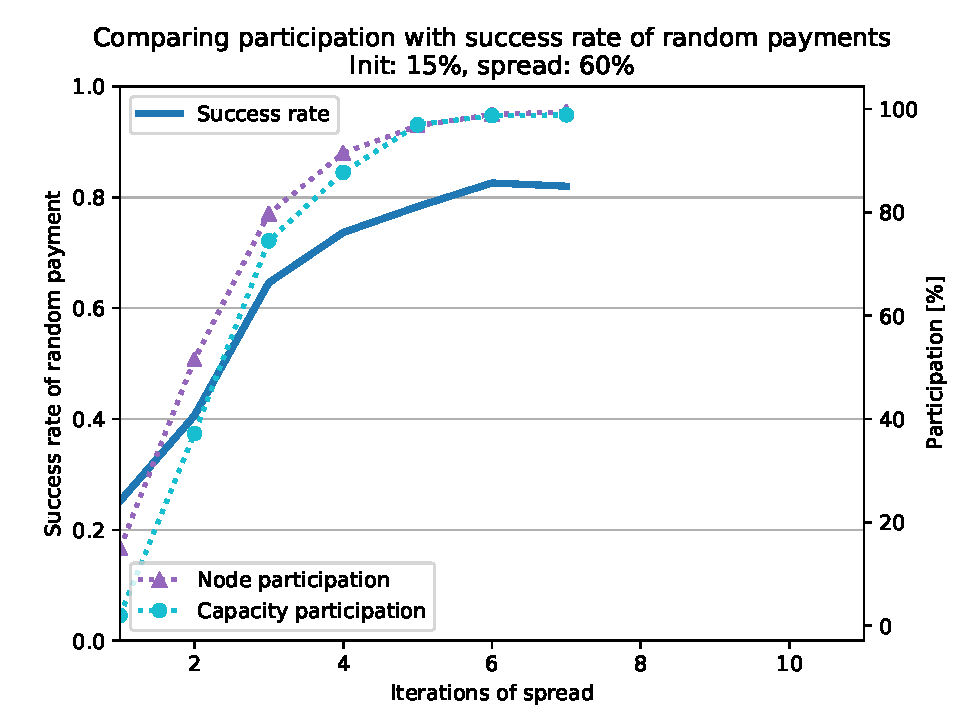
\includegraphics[width=60mm]{3a65a961_successrate_vs_participation_netw_spread_15_60.pdf}  \\
  (g) Init: 2 Spread: 60  & (h) Init: 10 Spread: 60 & (i) Init: 15 Spread: 60  \\[6pt]
\end{tabular}
\caption{Success Rate}
\end{figure}

\newpage 
\begin{figure}
\begin{tabular}{ccc}
  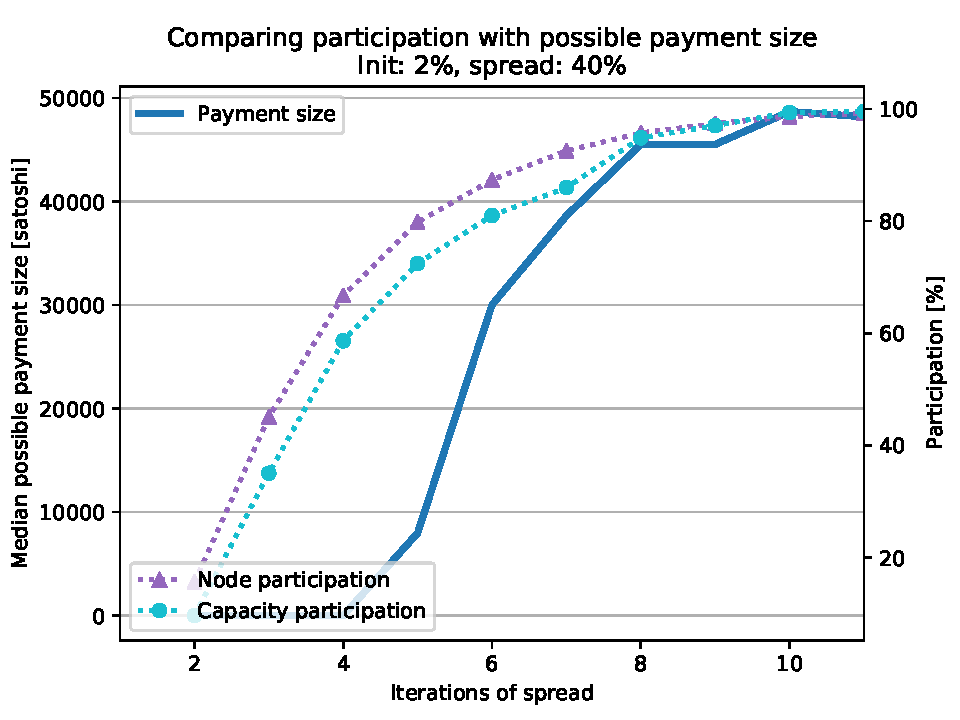
\includegraphics[width=60mm]{3a65a961_median_paymnet_size_vs_participation_netw_spread_02_40.pdf} &   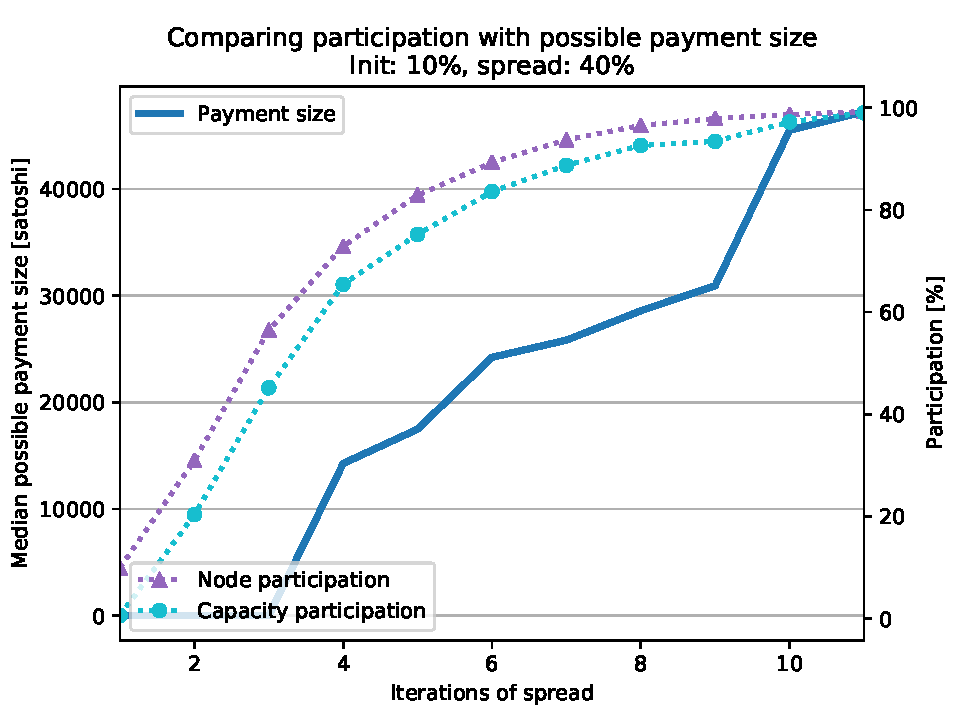
\includegraphics[width=60mm]{3a65a961_median_paymnet_size_vs_participation_netw_spread_10_40.pdf} & 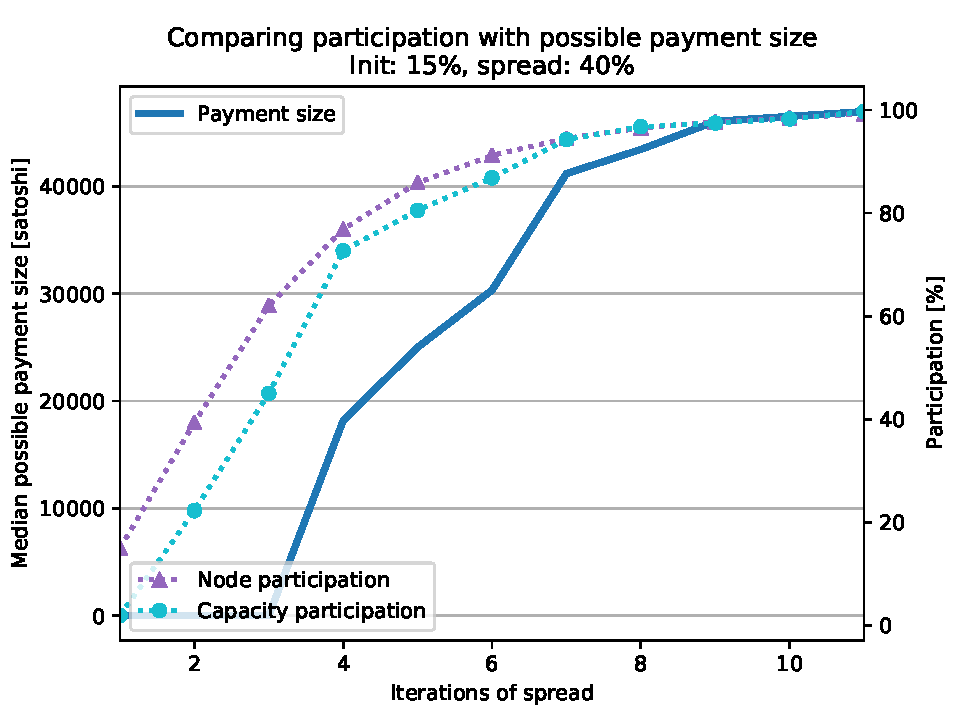
\includegraphics[width=60mm]{3a65a961_median_paymnet_size_vs_participation_netw_spread_15_40.pdf}  \\
  (a) Init: 2 Spread: 40  & (b) Init: 10 Spread: 40 & (c) Init: 15 Spread: 40  \\[6pt]
  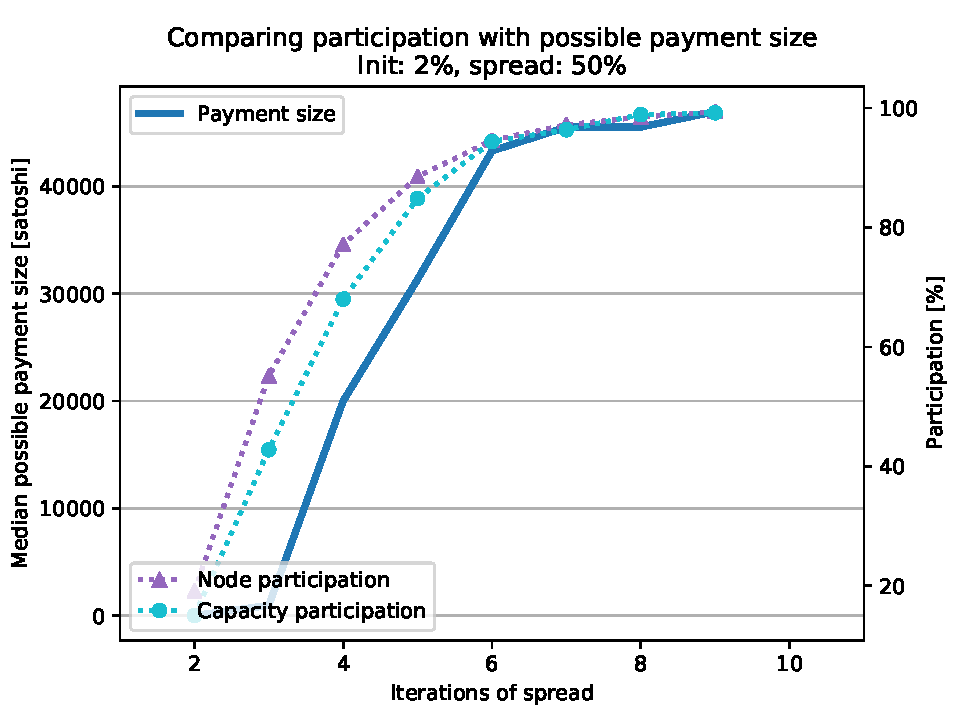
\includegraphics[width=60mm]{3a65a961_median_paymnet_size_vs_participation_netw_spread_02_50.pdf} &   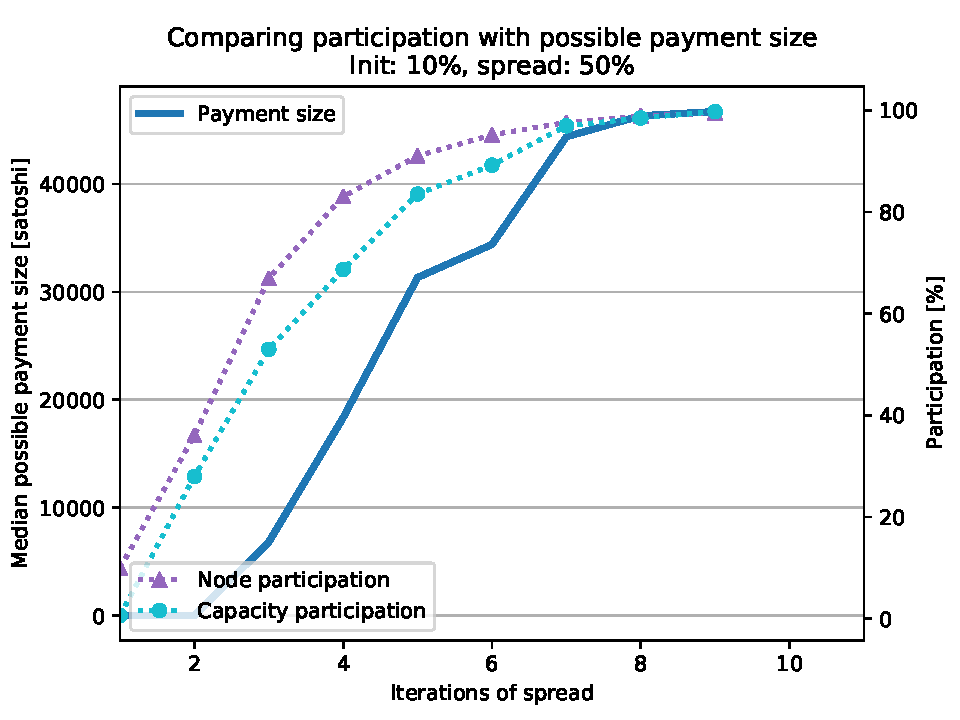
\includegraphics[width=60mm]{3a65a961_median_paymnet_size_vs_participation_netw_spread_10_50.pdf} & 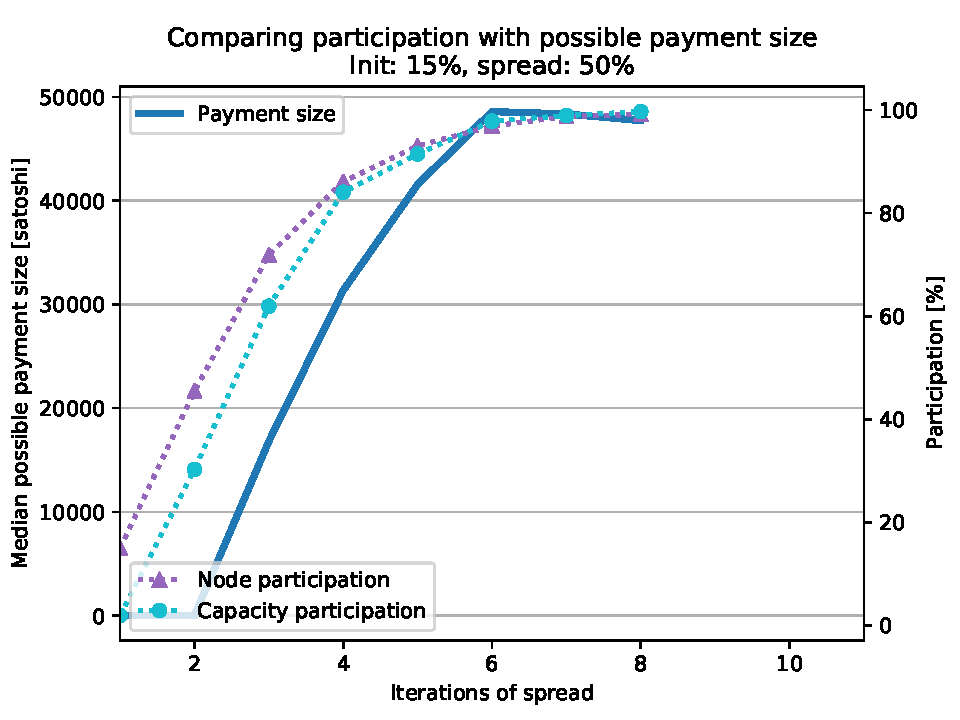
\includegraphics[width=60mm]{3a65a961_median_paymnet_size_vs_participation_netw_spread_15_50.pdf}  \\
  (d) Init: 2 Spread: 50  & (e) Init: 10 Spread: 50 & (f) Init: 15 Spread: 50  \\[6pt]
  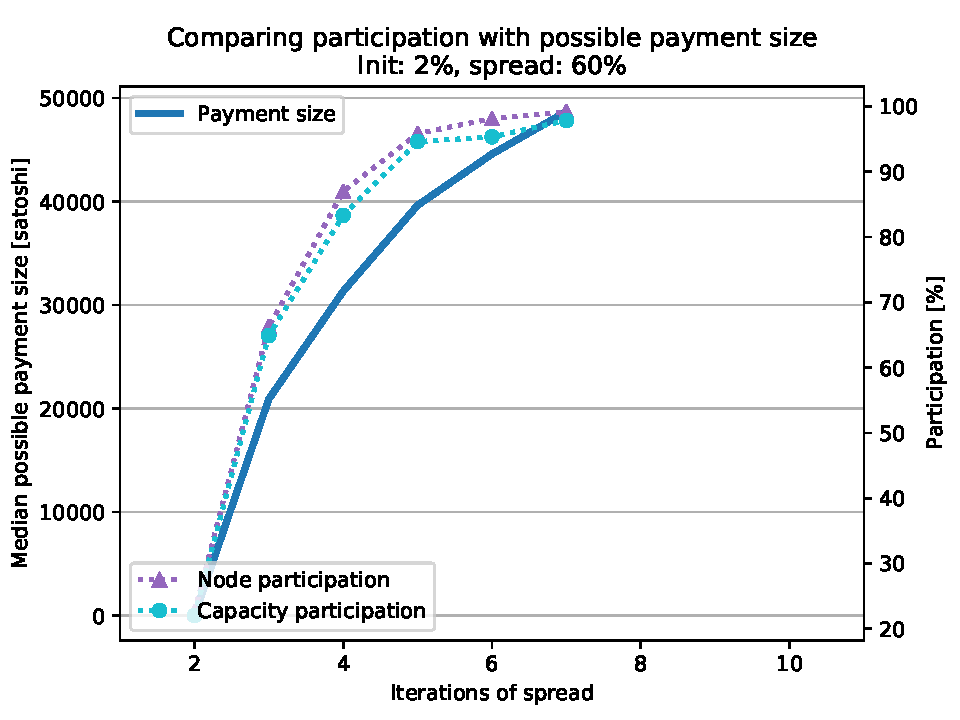
\includegraphics[width=60mm]{3a65a961_median_paymnet_size_vs_participation_netw_spread_02_60.pdf} &   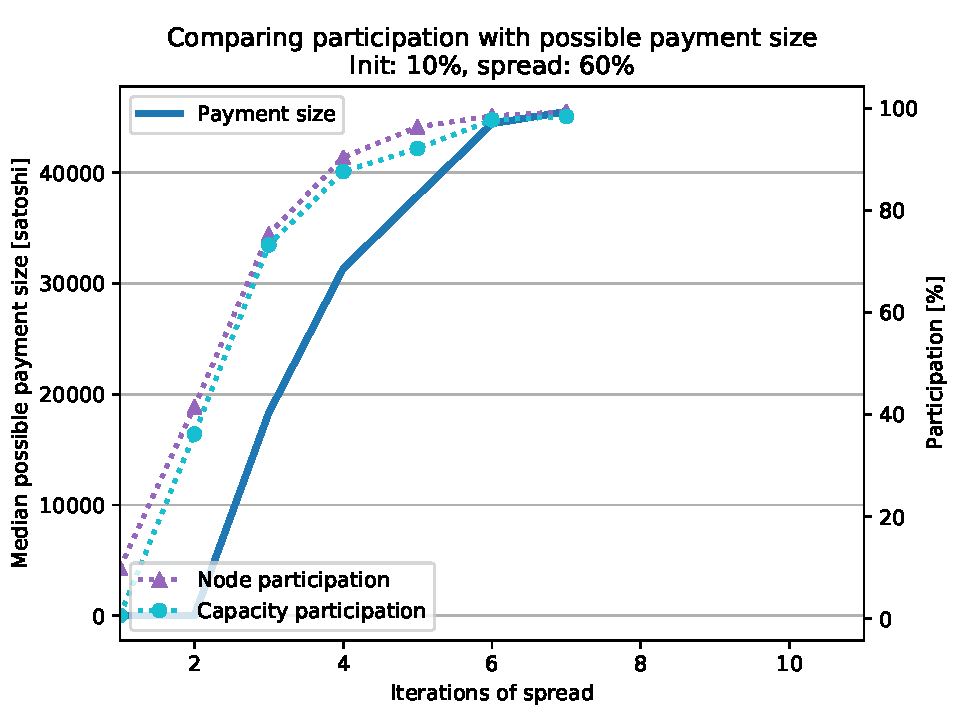
\includegraphics[width=60mm]{3a65a961_median_paymnet_size_vs_participation_netw_spread_10_60.pdf} & 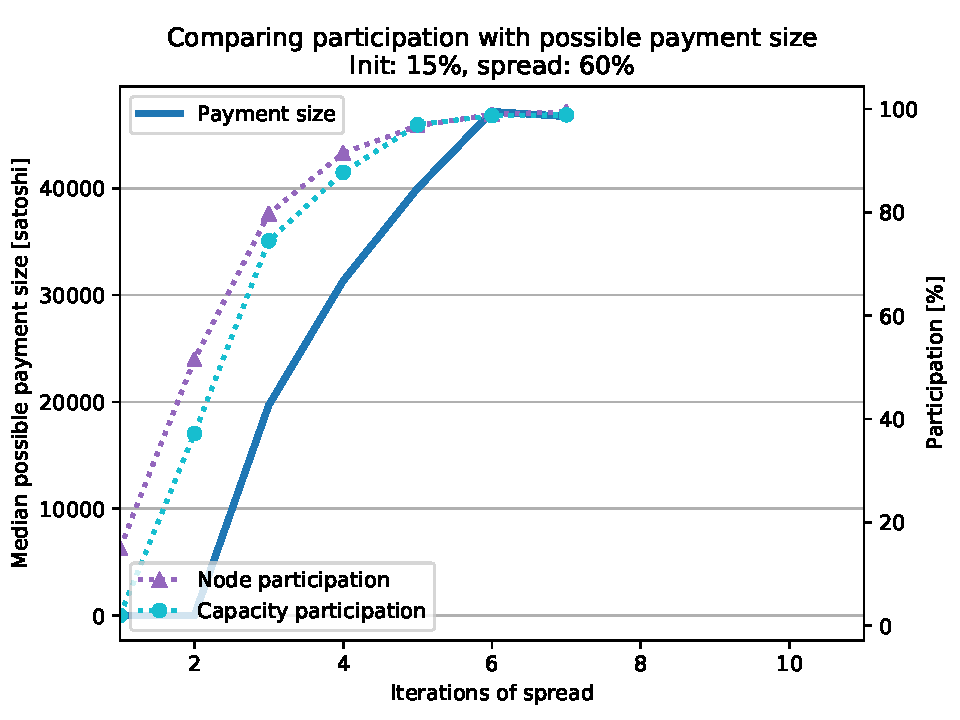
\includegraphics[width=60mm]{3a65a961_median_paymnet_size_vs_participation_netw_spread_15_60.pdf}  \\
  (g) Init: 2 Spread: 60  & (h) Init: 10 Spread: 60 & (i) Init: 15 Spread: 60  \\[6pt]
\end{tabular}
\caption{Median possible payment size}
\end{figure}

\newpage 
\begin{figure}
\begin{tabular}{ccc}
  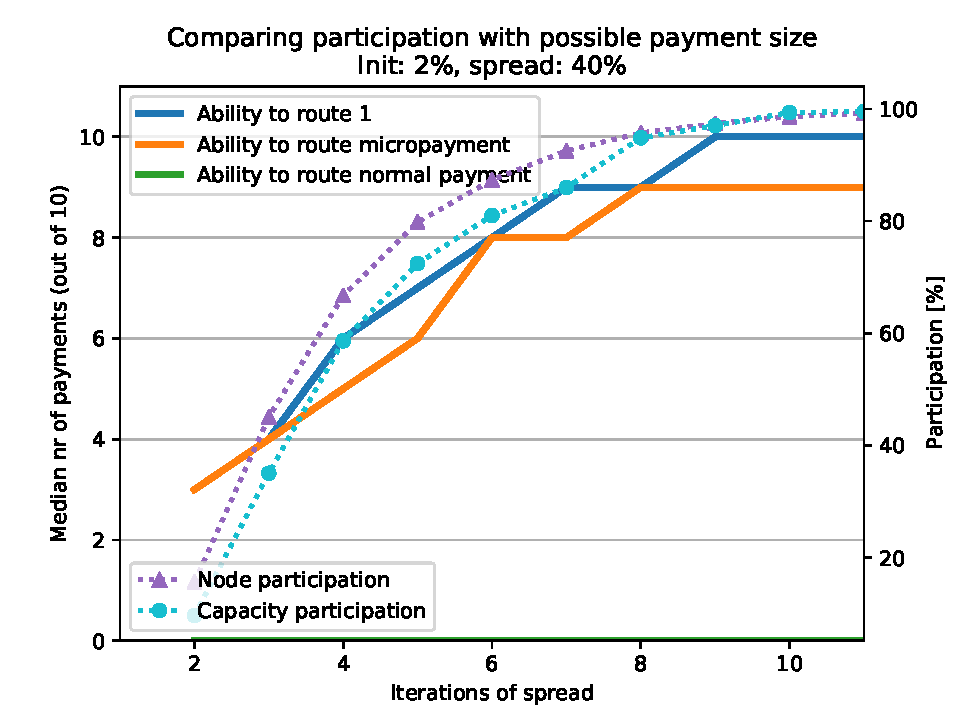
\includegraphics[width=60mm]{3a65a961_median_paymnets_vs_participation_netw_spread_02_40.pdf} &   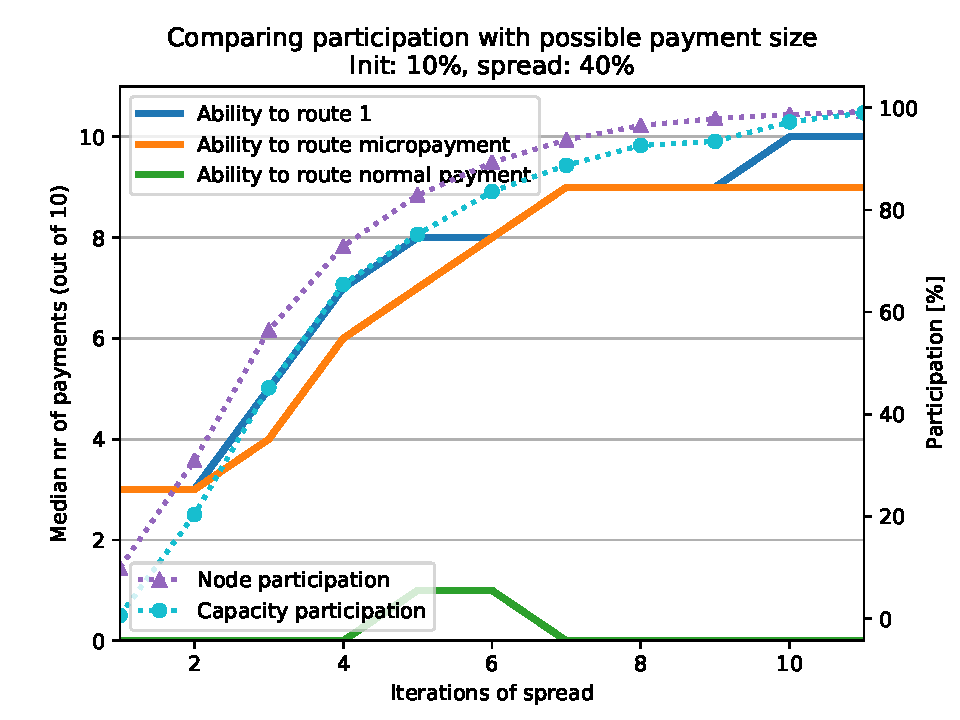
\includegraphics[width=60mm]{3a65a961_median_paymnets_vs_participation_netw_spread_10_40.pdf} & 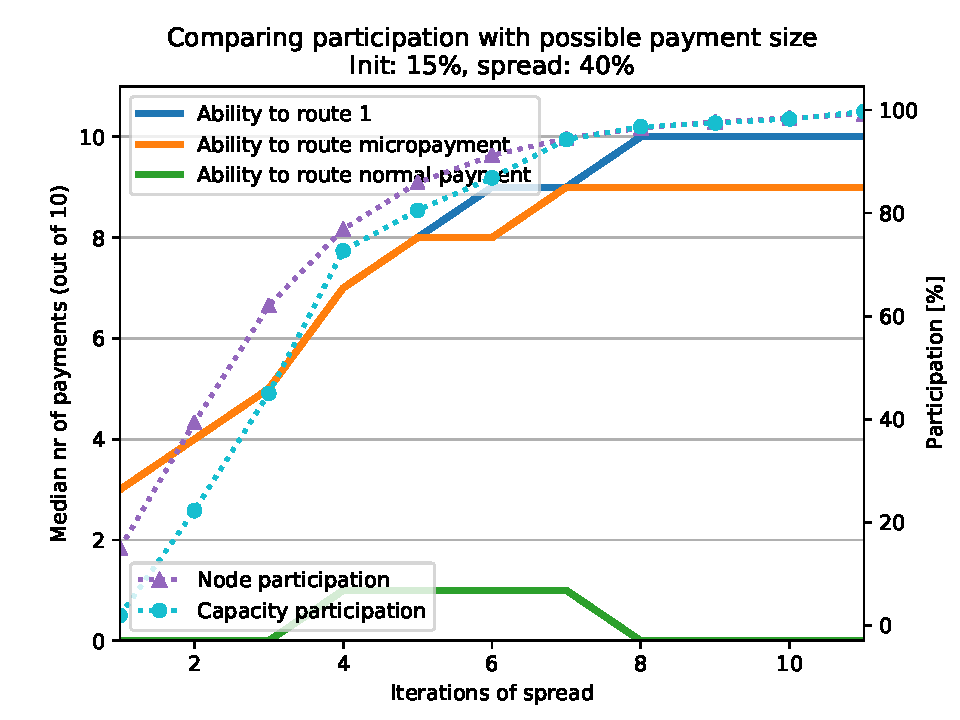
\includegraphics[width=60mm]{3a65a961_median_paymnets_vs_participation_netw_spread_15_40.pdf}  \\
  (a) Init: 2 Spread: 40  & (b) Init: 10 Spread: 40 & (c) Init: 15 Spread: 40  \\[6pt]
  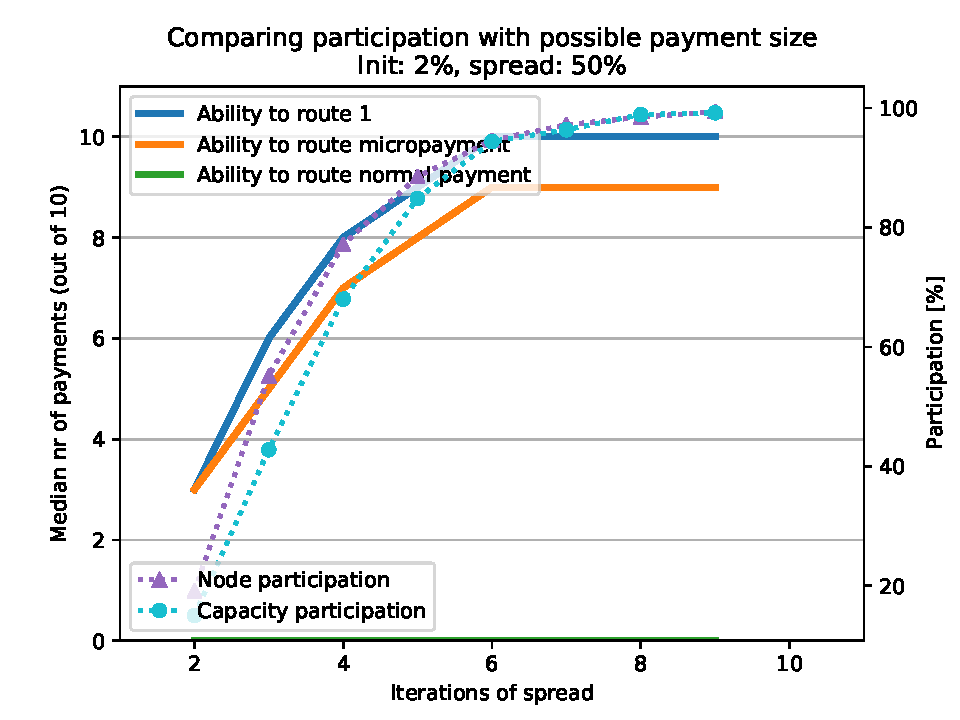
\includegraphics[width=60mm]{3a65a961_median_paymnets_vs_participation_netw_spread_02_50.pdf} &   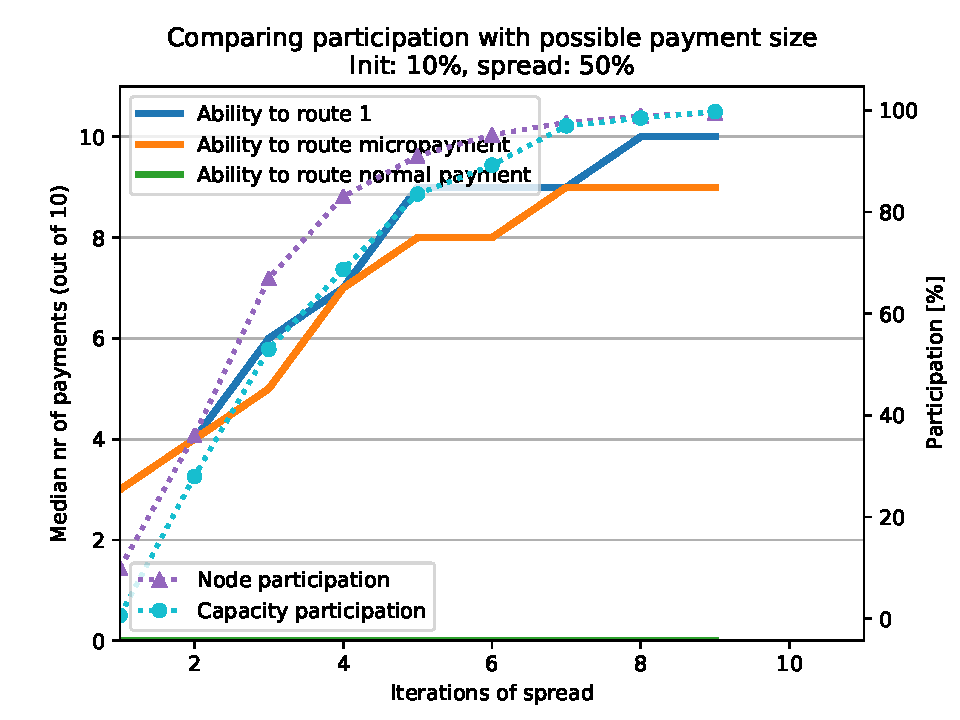
\includegraphics[width=60mm]{3a65a961_median_paymnets_vs_participation_netw_spread_10_50.pdf} & 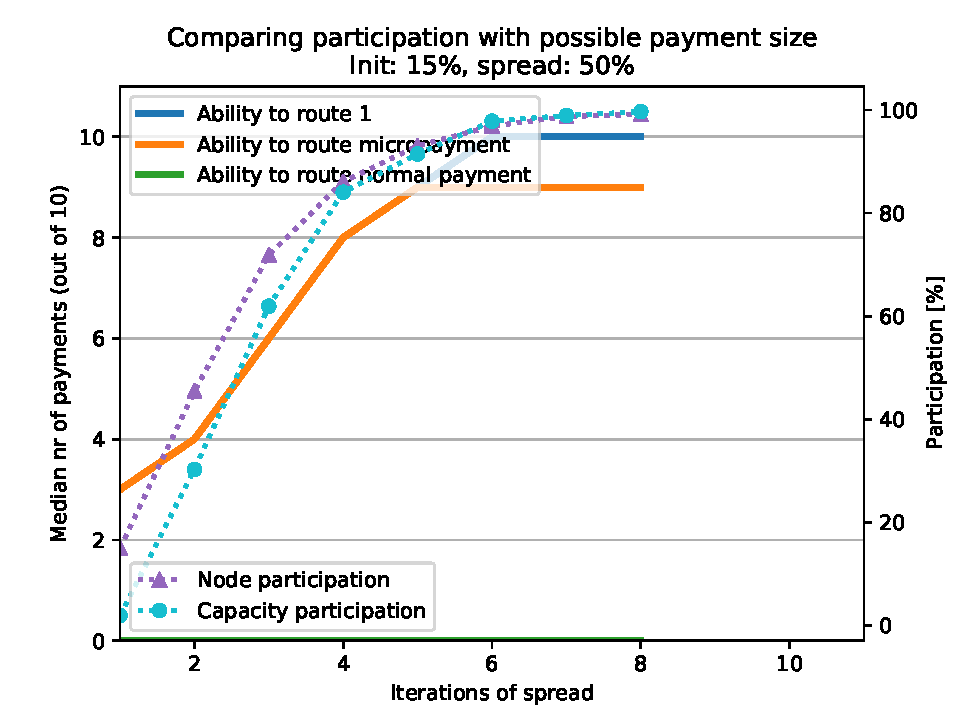
\includegraphics[width=60mm]{3a65a961_median_paymnets_vs_participation_netw_spread_15_50.pdf}  \\
  (d) Init: 2 Spread: 50  & (e) Init: 10 Spread: 50 & (f) Init: 15 Spread: 50  \\[6pt]
  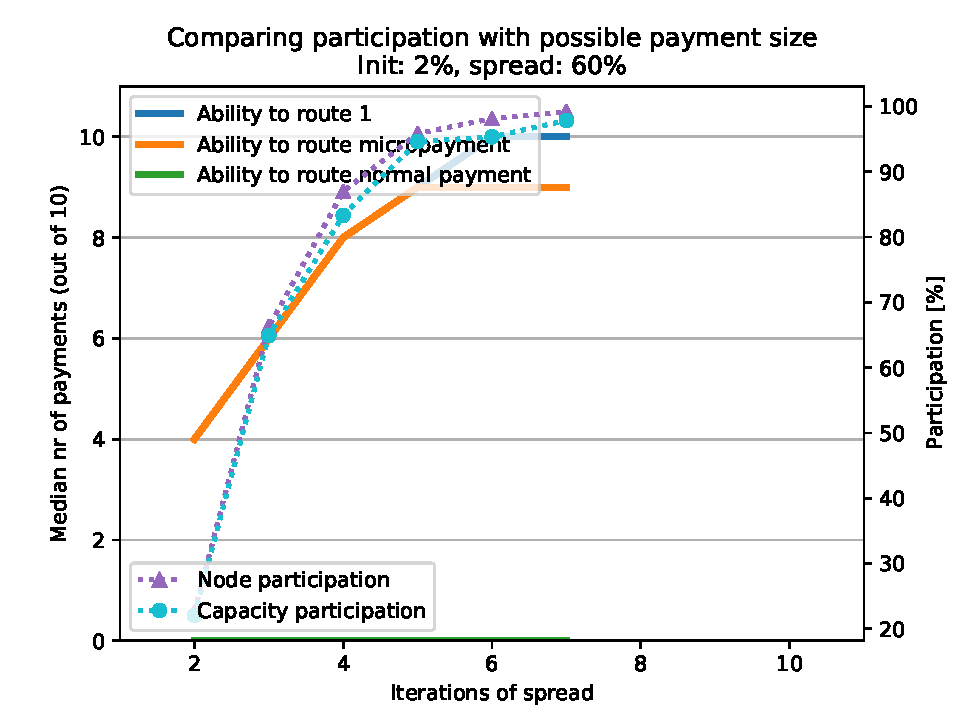
\includegraphics[width=60mm]{3a65a961_median_paymnets_vs_participation_netw_spread_02_60.pdf} &   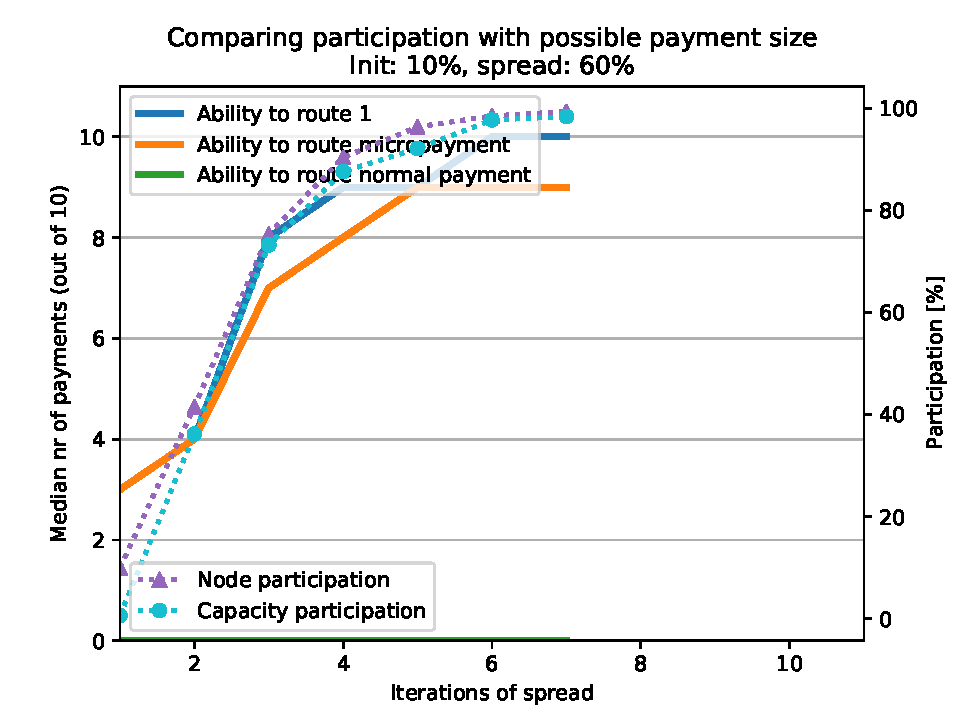
\includegraphics[width=60mm]{3a65a961_median_paymnets_vs_participation_netw_spread_10_60.pdf} & 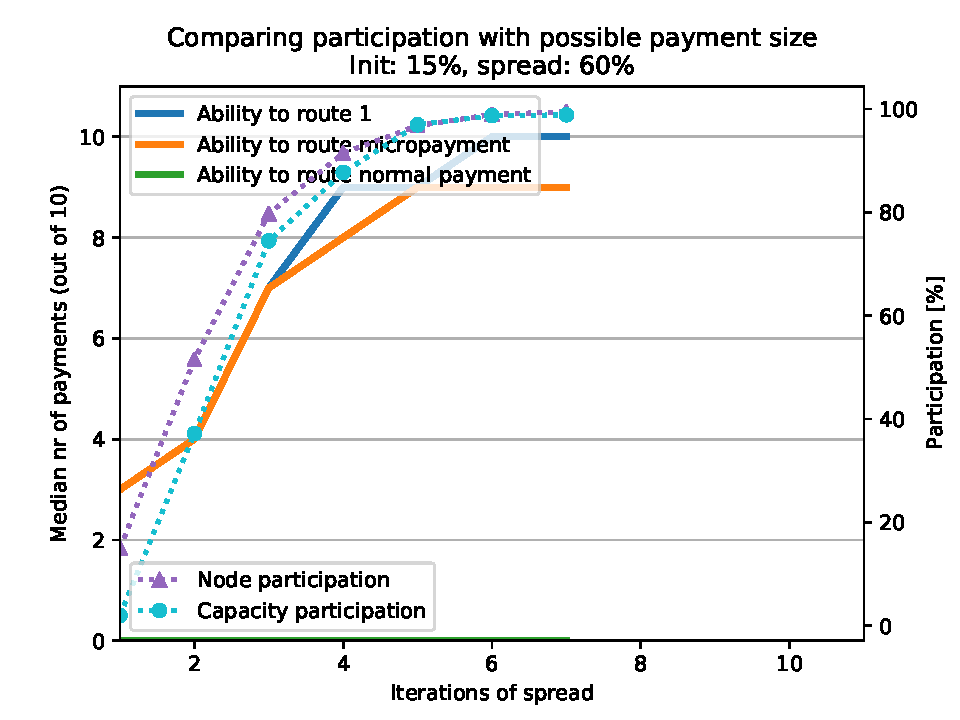
\includegraphics[width=60mm]{3a65a961_median_paymnets_vs_participation_netw_spread_15_60.pdf}  \\
  (g) Init: 2 Spread: 60  & (h) Init: 10 Spread: 60 & (i) Init: 15 Spread: 60  \\[6pt]
\end{tabular}
\caption{Different payment sizes}
\end{figure}

\newpage 
\begin{figure}
\begin{tabular}{ccc}
  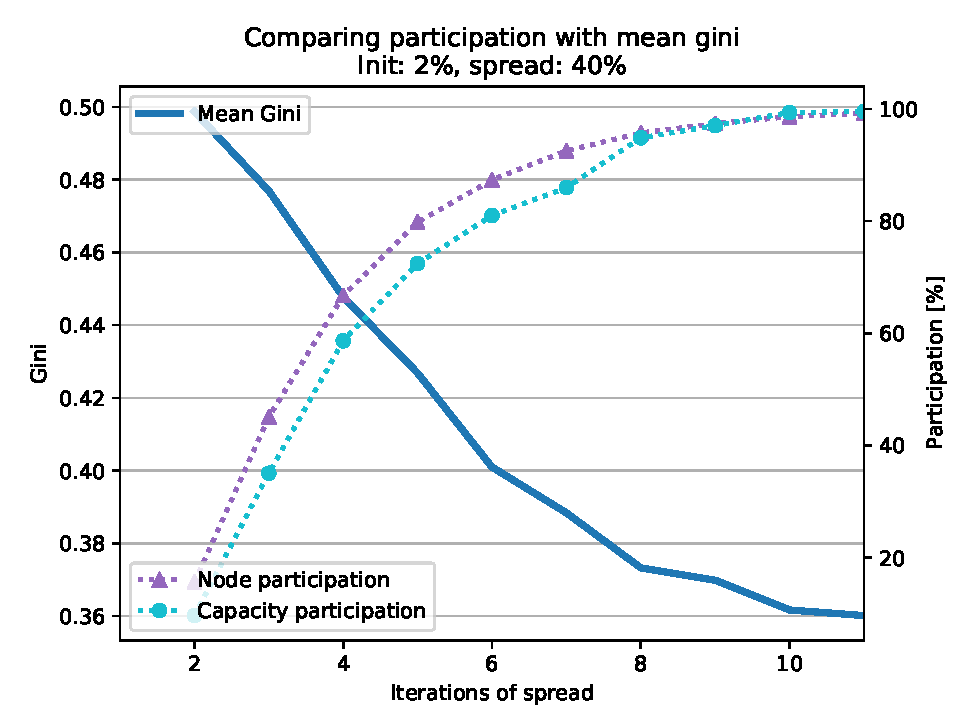
\includegraphics[width=60mm]{3a65a961_gini_vs_participation_netw_spread_02_40.pdf} &   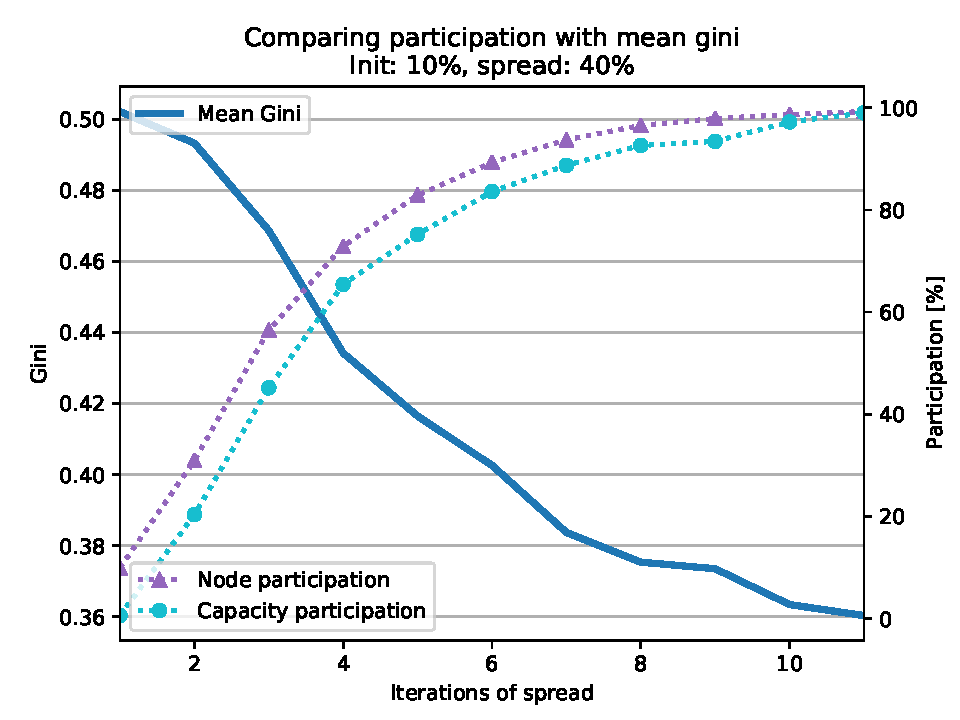
\includegraphics[width=60mm]{3a65a961_gini_vs_participation_netw_spread_10_40.pdf} & 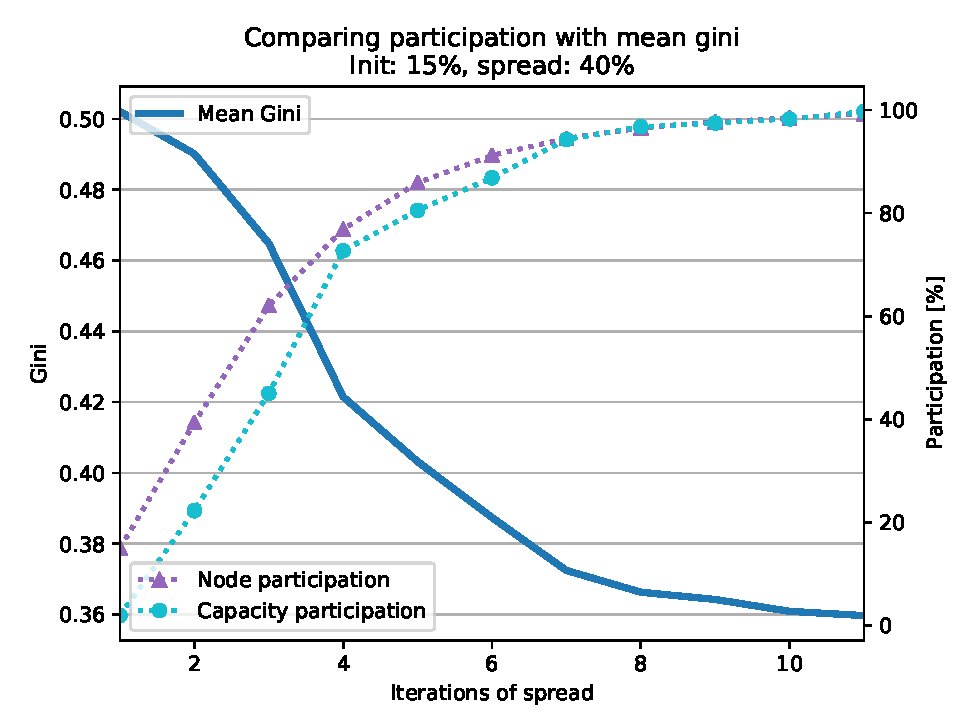
\includegraphics[width=60mm]{3a65a961_gini_vs_participation_netw_spread_15_40.pdf}  \\
  (a) Init: 2 Spread: 40  & (b) Init: 10 Spread: 40 & (c) Init: 15 Spread: 40  \\[6pt]
  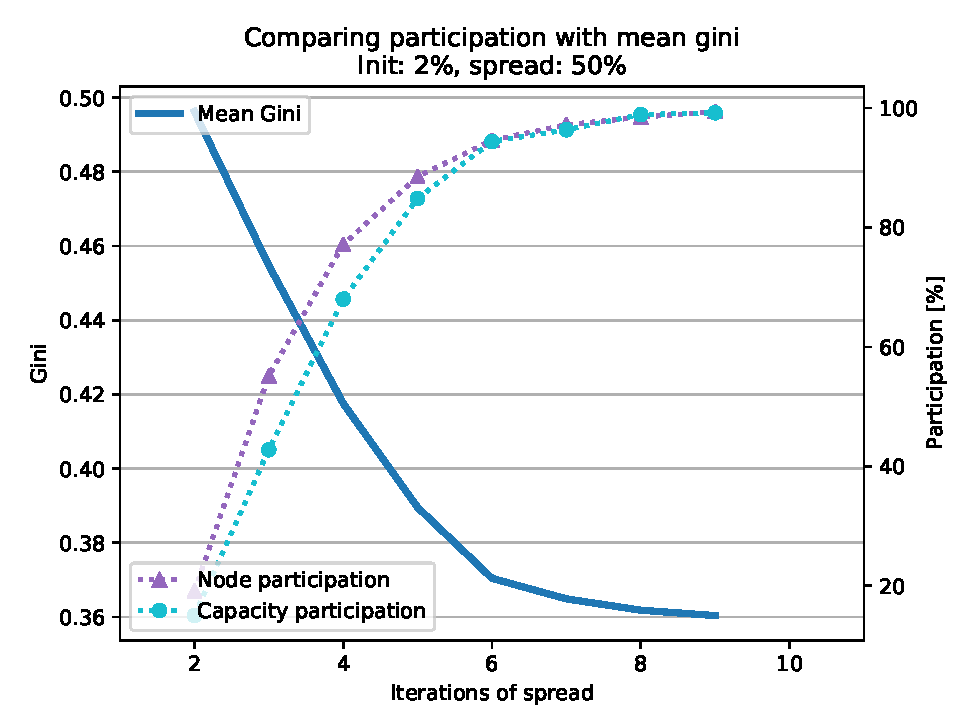
\includegraphics[width=60mm]{3a65a961_gini_vs_participation_netw_spread_02_50.pdf} &   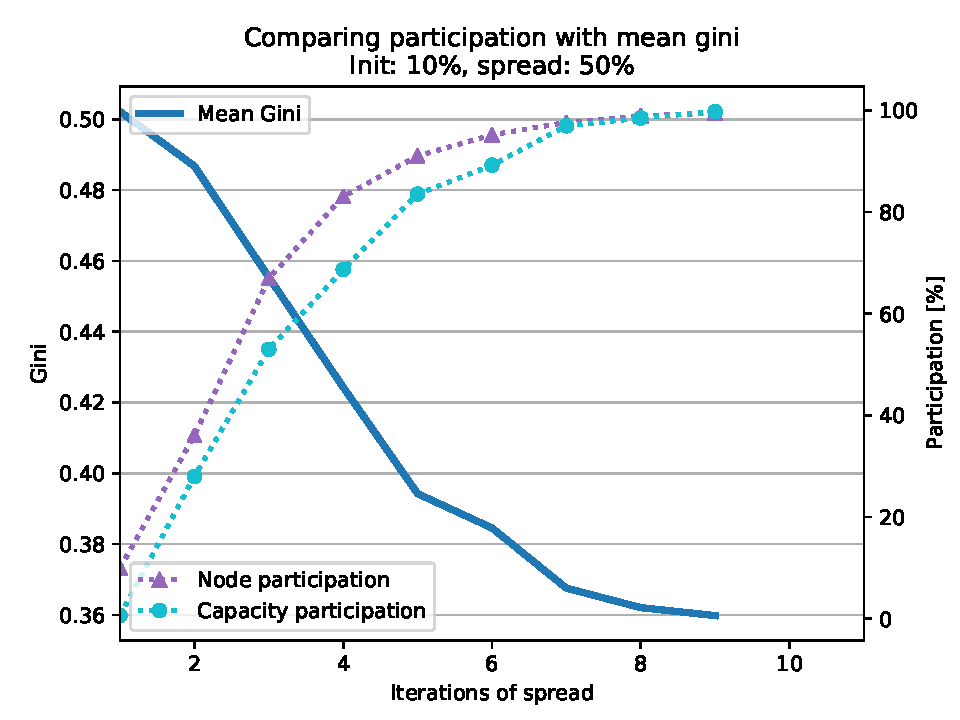
\includegraphics[width=60mm]{3a65a961_gini_vs_participation_netw_spread_10_50.pdf} & 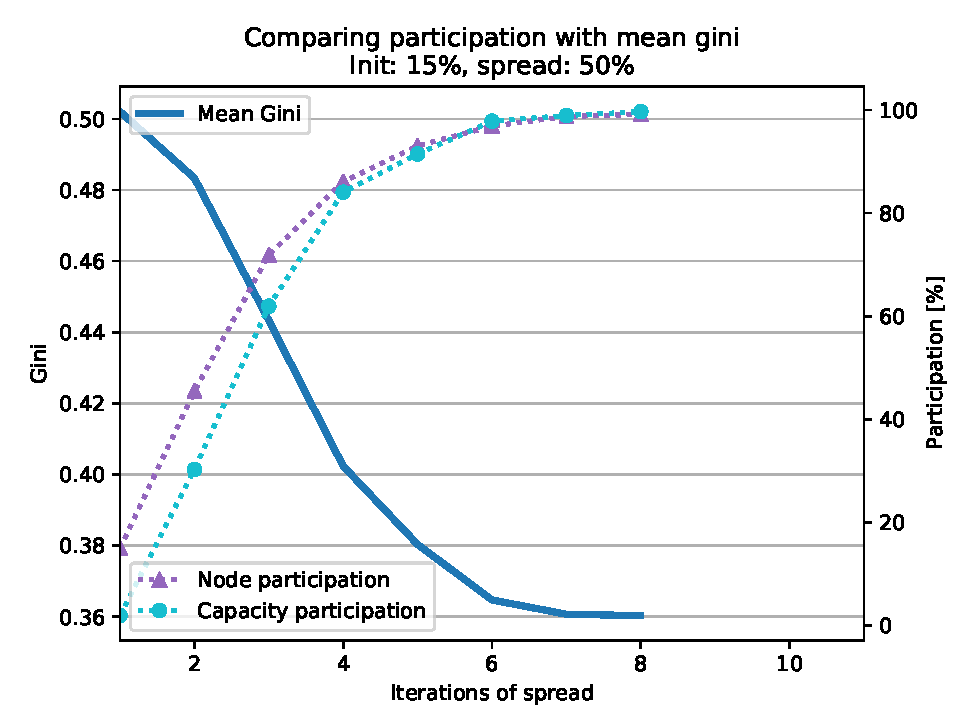
\includegraphics[width=60mm]{3a65a961_gini_vs_participation_netw_spread_15_50.pdf}  \\
  (d) Init: 2 Spread: 50  & (e) Init: 10 Spread: 50 & (f) Init: 15 Spread: 50  \\[6pt]
  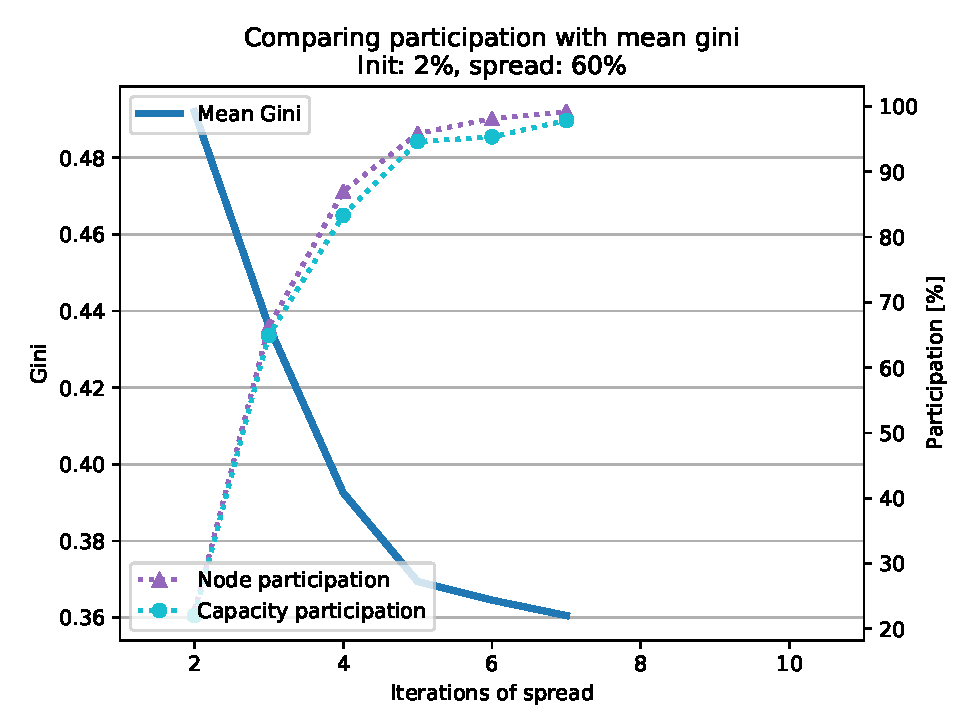
\includegraphics[width=60mm]{3a65a961_gini_vs_participation_netw_spread_02_60.pdf} &   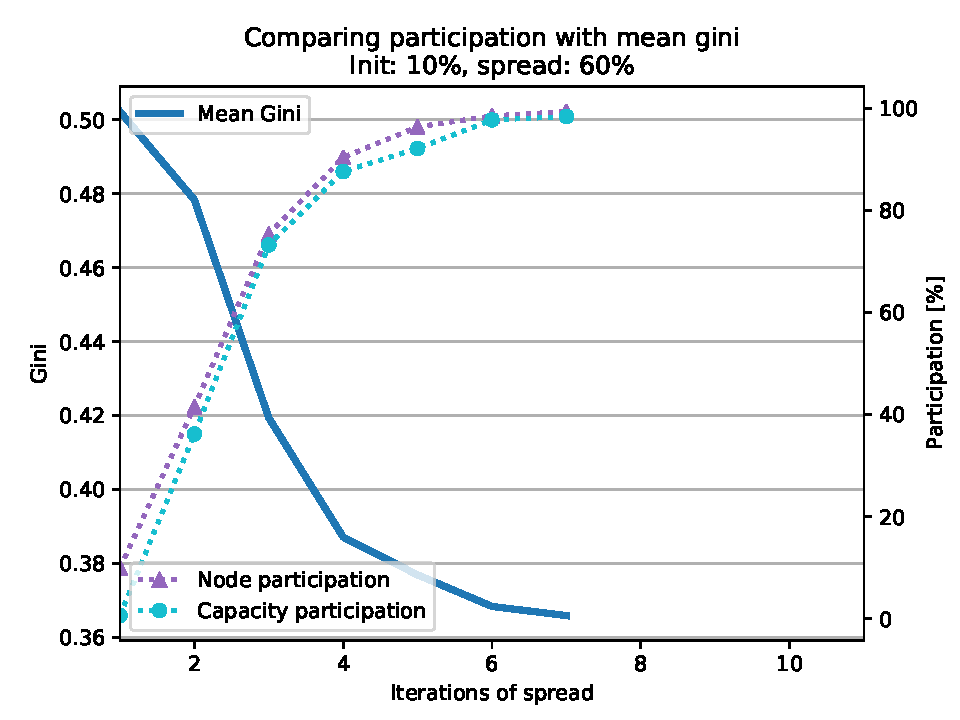
\includegraphics[width=60mm]{3a65a961_gini_vs_participation_netw_spread_10_60.pdf} & 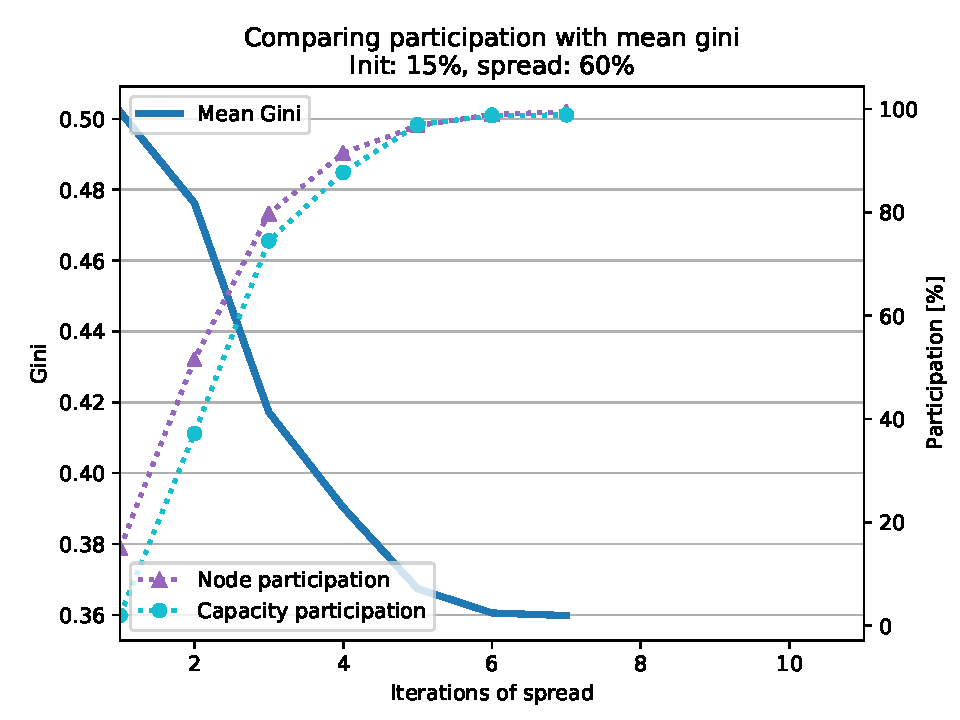
\includegraphics[width=60mm]{3a65a961_gini_vs_participation_netw_spread_15_60.pdf}  \\
  (g) Init: 2 Spread: 60  & (h) Init: 10 Spread: 60 & (i) Init: 15 Spread: 60  \\[6pt]
%\multicolumn{2}{c}{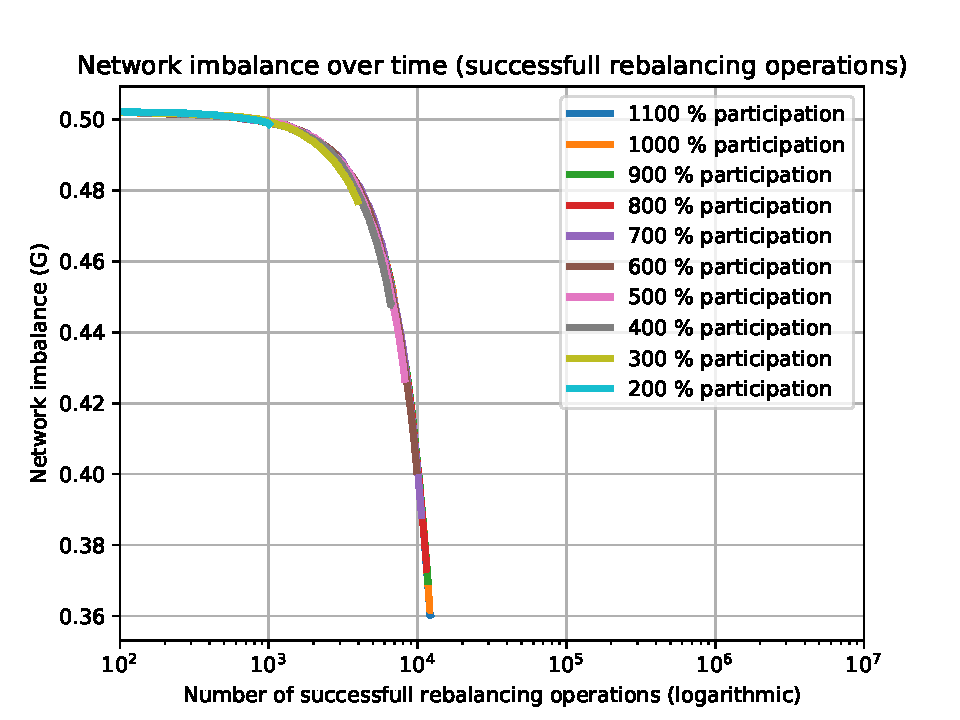
\includegraphics[width=60mm]{3a65a961_gini_vs_rebalops_netw_spread_02_40.pdf} }\\
%\multicolumn{2}{c}{(e) fifth}
\end{tabular}
\caption{Different payment sizes}
\end{figure}
\restoregeometry

\section{Conclusion \& Outlook}
%% Dummy text

%%---BIBLIOGRAPHY------------------------------------------------------------------------
\newpage
{\sloppypar
\printbibliography[heading=bibintoc]
\label{sec:lit}
}


%Print the glossary
\newpage
\newglossaryentry{doublespend}{
	name={double spend problem},
	description={Problem in digital cash systems that a digital token can be duplicated at will and used as payment to multiple receivers at the same time making it difficult to detect the fraud.}
}
\section*{Glossary}
\printglossaries

\appendix
\section{Some appendix}
maybe\ldots

%%---TODO-OVERVIEW-------------------
\ifdraft{%Do this only if mode=draft
\newpage
\listoftodos[\section{Todo-Notes}]
\clearpage
}
{%Do this only if mode=final
}

\end{document}

